\documentclass[1p]{elsarticle_modified}
%\bibliographystyle{elsarticle-num}

%\usepackage[colorlinks]{hyperref}
%\usepackage{abbrmath_seonhwa} %\Abb, \Ascr, \Acal ,\Abf, \Afrak
\usepackage{amsfonts}
\usepackage{amssymb}
\usepackage{amsmath}
\usepackage{amsthm}
\usepackage{scalefnt}
\usepackage{amsbsy}
\usepackage{kotex}
\usepackage{caption}
\usepackage{subfig}
\usepackage{color}
\usepackage{graphicx}
\usepackage{xcolor} %% white, black, red, green, blue, cyan, magenta, yellow
\usepackage{float}
\usepackage{setspace}
\usepackage{hyperref}

\usepackage{tikz}
\usetikzlibrary{arrows}

\usepackage{multirow}
\usepackage{array} % fixed length table
\usepackage{hhline}

%%%%%%%%%%%%%%%%%%%%%
\makeatletter
\renewcommand*\env@matrix[1][\arraystretch]{%
	\edef\arraystretch{#1}%
	\hskip -\arraycolsep
	\let\@ifnextchar\new@ifnextchar
	\array{*\c@MaxMatrixCols c}}
\makeatother %https://tex.stackexchange.com/questions/14071/how-can-i-increase-the-line-spacing-in-a-matrix
%%%%%%%%%%%%%%%

\usepackage[normalem]{ulem}

\newcommand{\msout}[1]{\ifmmode\text{\sout{\ensuremath{#1}}}\else\sout{#1}\fi}
%SOURCE: \msout is \stkout macro in https://tex.stackexchange.com/questions/20609/strikeout-in-math-mode

\newcommand{\cancel}[1]{
	\ifmmode
	{\color{red}\msout{#1}}
	\else
	{\color{red}\sout{#1}}
	\fi
}

\newcommand{\add}[1]{
	{\color{blue}\uwave{#1}}
}

\newcommand{\replace}[2]{
	\ifmmode
	{\color{red}\msout{#1}}{\color{blue}\uwave{#2}}
	\else
	{\color{red}\sout{#1}}{\color{blue}\uwave{#2}}
	\fi
}

\newcommand{\Sol}{\mathcal{S}} %segment
\newcommand{\D}{D} %diagram
\newcommand{\A}{\mathcal{A}} %arc


%%%%%%%%%%%%%%%%%%%%%%%%%%%%%5 test

\def\sl{\operatorname{\textup{SL}}(2,\Cbb)}
\def\psl{\operatorname{\textup{PSL}}(2,\Cbb)}
\def\quan{\mkern 1mu \triangleright \mkern 1mu}

\theoremstyle{definition}
\newtheorem{thm}{Theorem}[section]
\newtheorem{prop}[thm]{Proposition}
\newtheorem{lem}[thm]{Lemma}
\newtheorem{ques}[thm]{Question}
\newtheorem{cor}[thm]{Corollary}
\newtheorem{defn}[thm]{Definition}
\newtheorem{exam}[thm]{Example}
\newtheorem{rmk}[thm]{Remark}
\newtheorem{alg}[thm]{Algorithm}

\newcommand{\I}{\sqrt{-1}}
\begin{document}

%\begin{frontmatter}
%
%\title{Boundary parabolic representations of knots up to 8 crossings}
%
%%% Group authors per affiliation:
%\author{Yunhi Cho} 
%\address{Department of Mathematics, University of Seoul, Seoul, Korea}
%\ead{yhcho@uos.ac.kr}
%
%
%\author{Seonhwa Kim} %\fnref{s_kim}}
%\address{Center for Geometry and Physics, Institute for Basic Science, Pohang, 37673, Korea}
%\ead{ryeona17@ibs.re.kr}
%
%\author{Hyuk Kim}
%\address{Department of Mathematical Sciences, Seoul National University, Seoul 08826, Korea}
%\ead{hyukkim@snu.ac.kr}
%
%\author{Seokbeom Yoon}
%\address{Department of Mathematical Sciences, Seoul National University, Seoul, 08826,  Korea}
%\ead{sbyoon15@snu.ac.kr}
%
%\begin{abstract}
%We find all boundary parabolic representation of knots up to 8 crossings.
%
%\end{abstract}
%\begin{keyword}
%    \MSC[2010] 57M25 
%\end{keyword}
%
%\end{frontmatter}

%\linenumbers
%\tableofcontents
%
\newcommand\colored[1]{\textcolor{white}{\rule[-0.35ex]{0.8em}{1.4ex}}\kern-0.8em\color{red} #1}%
%\newcommand\colored[1]{\textcolor{white}{ #1}\kern-2.17ex	\textcolor{white}{ #1}\kern-1.81ex	\textcolor{white}{ #1}\kern-2.15ex\color{red}#1	}

{\Large $\underline{12a_{1076}~(K12a_{1076})}$}

\setlength{\tabcolsep}{10pt}
\renewcommand{\arraystretch}{1.6}
\vspace{1cm}\begin{tabular}{m{100pt}>{\centering\arraybackslash}m{274pt}}
\multirow{5}{120pt}{
	\centering
	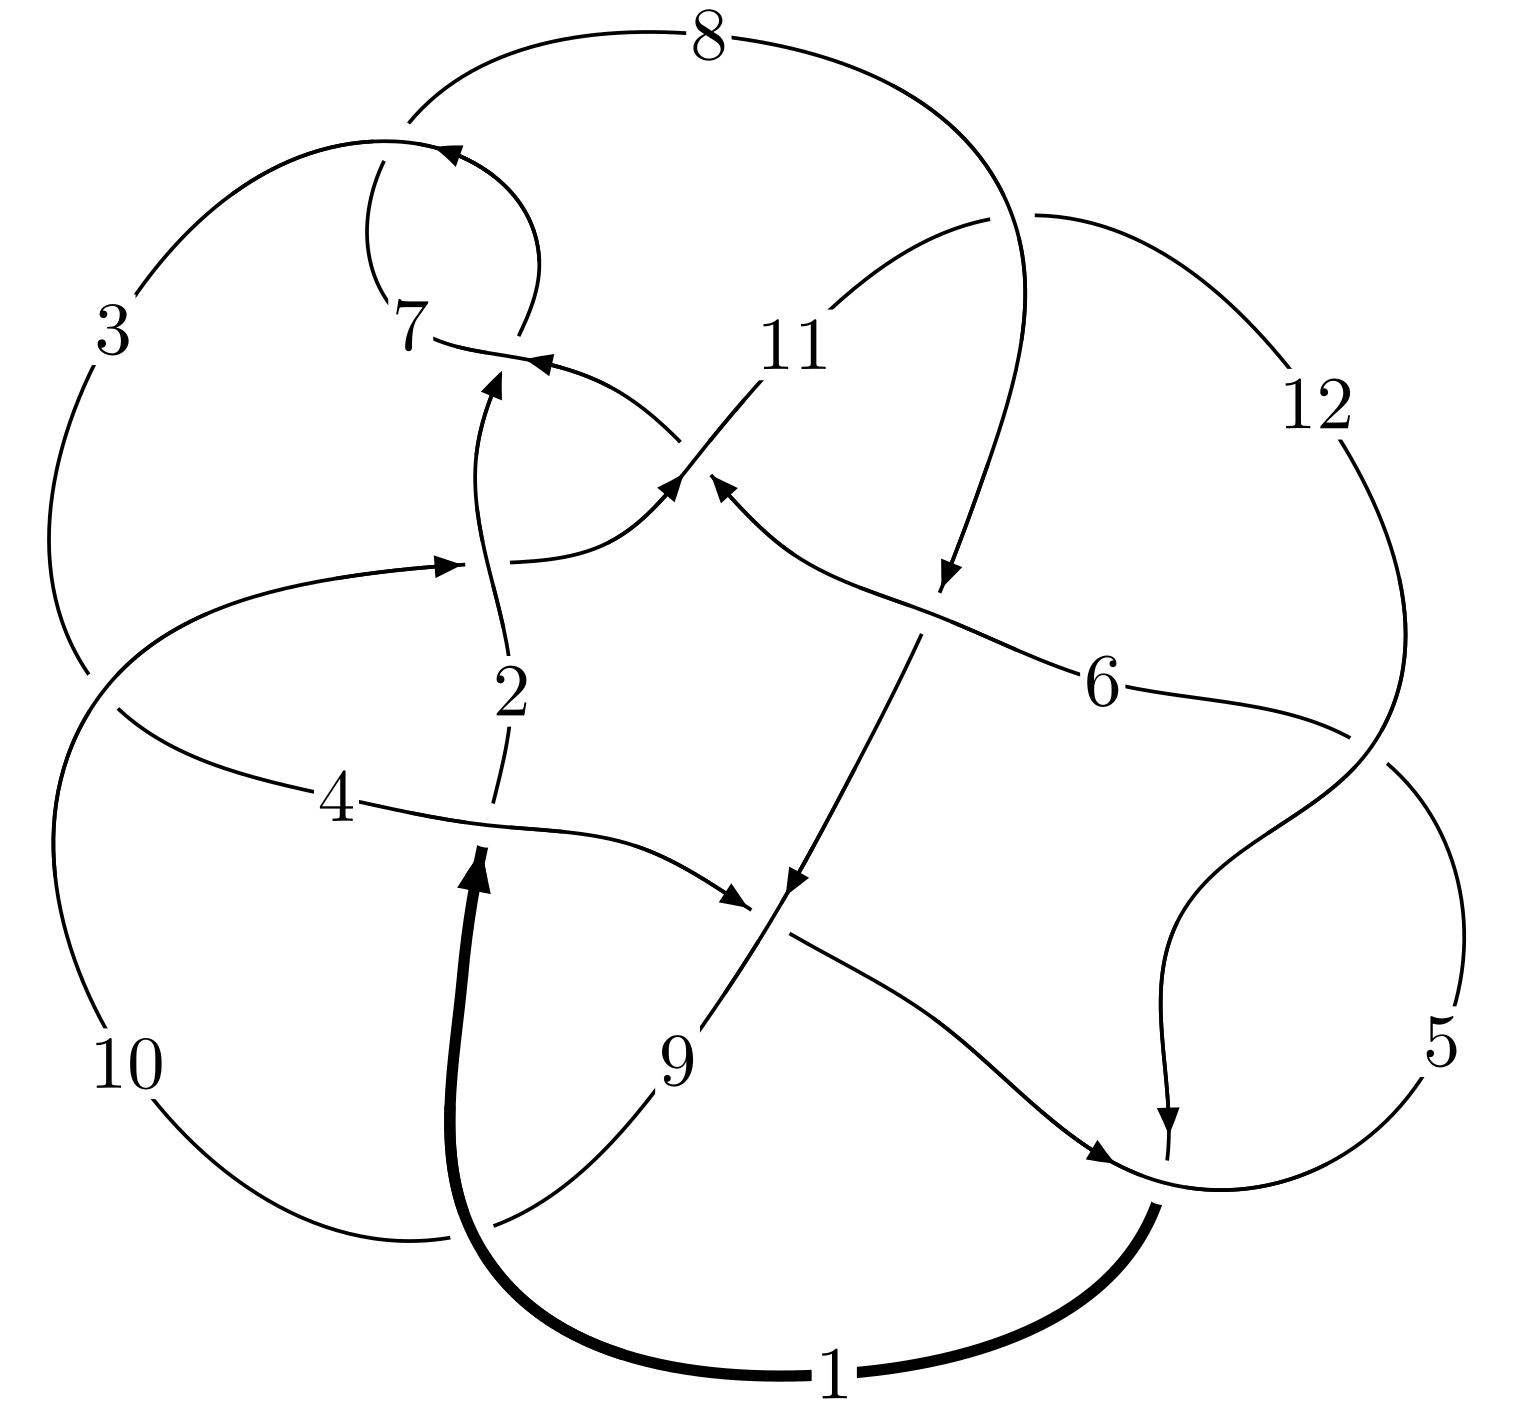
\includegraphics[width=112pt]{../../../GIT/diagram.site/Diagrams/png/1877_12a_1076.png}\\
\ \ \ A knot diagram\footnotemark}&
\allowdisplaybreaks
\textbf{Linearized knot diagam} \\
\cline{2-2}
 &
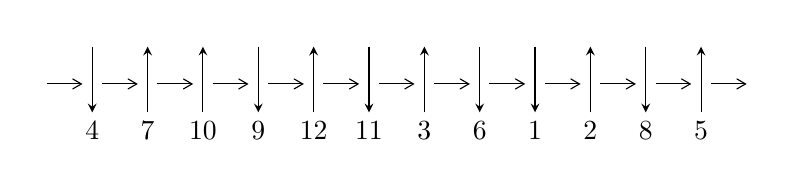
\begin{tikzpicture}[x=20pt, y=17pt]
	% nodes
	\node (C0) at (0, 0) {};
	\node (C1) at (1, 0) {};
	\node (C1U) at (1, +1) {};
	\node (C1D) at (1, -1) {4};

	\node (C2) at (2, 0) {};
	\node (C2U) at (2, +1) {};
	\node (C2D) at (2, -1) {7};

	\node (C3) at (3, 0) {};
	\node (C3U) at (3, +1) {};
	\node (C3D) at (3, -1) {10};

	\node (C4) at (4, 0) {};
	\node (C4U) at (4, +1) {};
	\node (C4D) at (4, -1) {9};

	\node (C5) at (5, 0) {};
	\node (C5U) at (5, +1) {};
	\node (C5D) at (5, -1) {12};

	\node (C6) at (6, 0) {};
	\node (C6U) at (6, +1) {};
	\node (C6D) at (6, -1) {11};

	\node (C7) at (7, 0) {};
	\node (C7U) at (7, +1) {};
	\node (C7D) at (7, -1) {3};

	\node (C8) at (8, 0) {};
	\node (C8U) at (8, +1) {};
	\node (C8D) at (8, -1) {6};

	\node (C9) at (9, 0) {};
	\node (C9U) at (9, +1) {};
	\node (C9D) at (9, -1) {1};

	\node (C10) at (10, 0) {};
	\node (C10U) at (10, +1) {};
	\node (C10D) at (10, -1) {2};

	\node (C11) at (11, 0) {};
	\node (C11U) at (11, +1) {};
	\node (C11D) at (11, -1) {8};

	\node (C12) at (12, 0) {};
	\node (C12U) at (12, +1) {};
	\node (C12D) at (12, -1) {5};
	\node (C13) at (13, 0) {};

	% arrows
	\draw[->,>={angle 60}]
	(C0) edge (C1) (C1) edge (C2) (C2) edge (C3) (C3) edge (C4) (C4) edge (C5) (C5) edge (C6) (C6) edge (C7) (C7) edge (C8) (C8) edge (C9) (C9) edge (C10) (C10) edge (C11) (C11) edge (C12) (C12) edge (C13) ;	\draw[->,>=stealth]
	(C1U) edge (C1D) (C2D) edge (C2U) (C3D) edge (C3U) (C4U) edge (C4D) (C5D) edge (C5U) (C6U) edge (C6D) (C7D) edge (C7U) (C8U) edge (C8D) (C9U) edge (C9D) (C10D) edge (C10U) (C11U) edge (C11D) (C12D) edge (C12U) ;
	\end{tikzpicture} \\
\hhline{~~} \\& 
\textbf{Solving Sequence} \\ \cline{2-2} 
 &
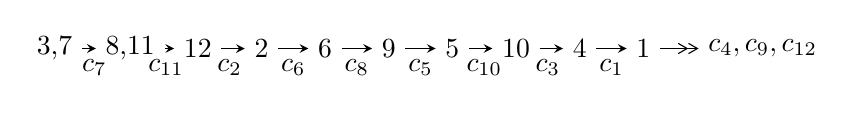
\begin{tikzpicture}[x=23pt, y=7pt]
	% node
	\node (A0) at (-1/8, 0) {3,7};
	\node (A1) at (17/16, 0) {8,11};
	\node (A2) at (17/8, 0) {12};
	\node (A3) at (25/8, 0) {2};
	\node (A4) at (33/8, 0) {6};
	\node (A5) at (41/8, 0) {9};
	\node (A6) at (49/8, 0) {5};
	\node (A7) at (57/8, 0) {10};
	\node (A8) at (65/8, 0) {4};
	\node (A9) at (73/8, 0) {1};
	\node (C1) at (1/2, -1) {$c_{7}$};
	\node (C2) at (13/8, -1) {$c_{11}$};
	\node (C3) at (21/8, -1) {$c_{2}$};
	\node (C4) at (29/8, -1) {$c_{6}$};
	\node (C5) at (37/8, -1) {$c_{8}$};
	\node (C6) at (45/8, -1) {$c_{5}$};
	\node (C7) at (53/8, -1) {$c_{10}$};
	\node (C8) at (61/8, -1) {$c_{3}$};
	\node (C9) at (69/8, -1) {$c_{1}$};
	\node (A10) at (11, 0) {$c_{4},c_{9},c_{12}$};

	% edge
	\draw[->,>=stealth]	
	(A0) edge (A1) (A1) edge (A2) (A2) edge (A3) (A3) edge (A4) (A4) edge (A5) (A5) edge (A6) (A6) edge (A7) (A7) edge (A8) (A8) edge (A9) ;
	\draw[->>,>={angle 60}]	
	(A9) edge (A10);
\end{tikzpicture} \\ 

\end{tabular} \\

\footnotetext{
The image of knot diagram is generated by the software ``\textbf{Draw programme}" developed by Andrew Bartholomew(\url{http://www.layer8.co.uk/maths/draw/index.htm\#Running-draw}), where we modified some parts for our purpose(\url{https://github.com/CATsTAILs/LinksPainter}).
}\phantom \\ \newline 
\centering \textbf{Ideals for irreducible components\footnotemark of $X_{\text{par}}$} 
 
\begin{align*}
I^u_{1}&=\langle 
-6.51635\times10^{1061} u^{177}-1.25795\times10^{1062} u^{176}+\cdots+1.40470\times10^{1063} b-8.65454\times10^{1066},\\
\phantom{I^u_{1}}&\phantom{= \langle  }1.48578\times10^{1069} u^{177}+3.21858\times10^{1069} u^{176}+\cdots+1.03497\times10^{1070} a+3.77579\times10^{1073},\\
\phantom{I^u_{1}}&\phantom{= \langle  }u^{178}+2 u^{177}+\cdots+2168879 u+237673\rangle \\
I^u_{2}&=\langle 
-3.12220\times10^{39} u^{41}-9.70960\times10^{39} u^{40}+\cdots+5.62023\times10^{39} b-9.01968\times10^{39},\\
\phantom{I^u_{2}}&\phantom{= \langle  }-9.07781\times10^{39} u^{41}-6.68667\times10^{39} u^{40}+\cdots+5.62023\times10^{39} a+1.34444\times10^{41},\;u^{42}+u^{41}+\cdots-3 u+1\rangle \\
\\
\end{align*}
\raggedright * 2 irreducible components of $\dim_{\mathbb{C}}=0$, with total 220 representations.\\
\footnotetext{All coefficients of polynomials are rational numbers. But the coefficients are sometimes approximated in decimal forms when there is not enough margin.}
\newpage
\renewcommand{\arraystretch}{1}
\centering \section*{I. $I^u_{1}= \langle -6.52\times10^{1061} u^{177}-1.26\times10^{1062} u^{176}+\cdots+1.40\times10^{1063} b-8.65\times10^{1066},\;1.49\times10^{1069} u^{177}+3.22\times10^{1069} u^{176}+\cdots+1.03\times10^{1070} a+3.78\times10^{1073},\;u^{178}+2 u^{177}+\cdots+2168879 u+237673 \rangle$}
\flushleft \textbf{(i) Arc colorings}\\
\begin{tabular}{m{7pt} m{180pt} m{7pt} m{180pt} }
\flushright $a_{3}=$&$\begin{pmatrix}0\\u\end{pmatrix}$ \\
\flushright $a_{7}=$&$\begin{pmatrix}1\\0\end{pmatrix}$ \\
\flushright $a_{8}=$&$\begin{pmatrix}1\\- u^2\end{pmatrix}$ \\
\flushright $a_{11}=$&$\begin{pmatrix}-0.143559 u^{177}-0.310985 u^{176}+\cdots-8706.70 u-3648.23\\0.0463895 u^{177}+0.0895526 u^{176}+\cdots+45107.3 u+6161.12\end{pmatrix}$ \\
\flushright $a_{12}=$&$\begin{pmatrix}-0.0399629 u^{177}-0.0548352 u^{176}+\cdots-139699. u-15481.9\\-0.0464781 u^{177}-0.137170 u^{176}+\cdots+175912. u+17797.0\end{pmatrix}$ \\
\flushright $a_{2}=$&$\begin{pmatrix}- u\\u\end{pmatrix}$ \\
\flushright $a_{6}=$&$\begin{pmatrix}0.0292828 u^{177}+0.154408 u^{176}+\cdots-245118. u-25864.2\\-0.0397983 u^{177}-0.178705 u^{176}+\cdots+263781. u+28156.8\end{pmatrix}$ \\
\flushright $a_{9}=$&$\begin{pmatrix}0.0216693 u^{177}+0.0288690 u^{176}+\cdots+95096.4 u+9916.14\\0.0161521 u^{177}+0.0822877 u^{176}+\cdots-235942. u-24443.3\end{pmatrix}$ \\
\flushright $a_{5}=$&$\begin{pmatrix}0.133434 u^{177}+0.388951 u^{176}+\cdots-345828. u-34551.6\\-0.0363532 u^{177}-0.123260 u^{176}+\cdots+109844. u+12057.4\end{pmatrix}$ \\
\flushright $a_{10}=$&$\begin{pmatrix}-0.0356100 u^{177}-0.0596208 u^{176}+\cdots-90563.5 u-10087.6\\-0.0615594 u^{177}-0.161811 u^{176}+\cdots+126964. u+12600.5\end{pmatrix}$ \\
\flushright $a_{4}=$&$\begin{pmatrix}0.115818 u^{177}+0.283079 u^{176}+\cdots-139607. u-11721.2\\-0.0477208 u^{177}-0.125972 u^{176}+\cdots+67851.1 u+6289.36\end{pmatrix}$ \\
\flushright $a_{1}=$&$\begin{pmatrix}-0.0872571 u^{177}-0.186760 u^{176}+\cdots+124086. u+10099.2\\0.00876483 u^{177}+0.0448885 u^{176}+\cdots-19193.0 u-2288.77\end{pmatrix}$\\&\end{tabular}
\flushleft \textbf{(ii) Obstruction class $= -1$}\\~\\
\flushleft \textbf{(iii) Cusp Shapes $= 0.125336 u^{177}+0.257783 u^{176}+\cdots-309492. u-30772.4$}\\~\\
\newpage\renewcommand{\arraystretch}{1}
\flushleft \textbf{(iv) u-Polynomials at the component}\newline \\
\begin{tabular}{m{50pt}|m{274pt}}
Crossings & \hspace{64pt}u-Polynomials at each crossing \\
\hline $$\begin{aligned}c_{1}\end{aligned}$$&$\begin{aligned}
&u^{178}-16 u^{177}+\cdots-605422 u+32771
\end{aligned}$\\
\hline $$\begin{aligned}c_{2},c_{7}\end{aligned}$$&$\begin{aligned}
&u^{178}+2 u^{177}+\cdots+2168879 u+237673
\end{aligned}$\\
\hline $$\begin{aligned}c_{3}\end{aligned}$$&$\begin{aligned}
&4(4 u^{178}+4 u^{177}+\cdots+938639 u+398051)
\end{aligned}$\\
\hline $$\begin{aligned}c_{4}\end{aligned}$$&$\begin{aligned}
&u^{178}+4 u^{177}+\cdots-416 u+16
\end{aligned}$\\
\hline $$\begin{aligned}c_{5},c_{12}\end{aligned}$$&$\begin{aligned}
&u^{178}-3 u^{177}+\cdots+80 u+1
\end{aligned}$\\
\hline $$\begin{aligned}c_{6}\end{aligned}$$&$\begin{aligned}
&4(4 u^{178}-24 u^{177}+\cdots-5.32279\times10^{8} u+2.88321\times10^{8})
\end{aligned}$\\
\hline $$\begin{aligned}c_{8}\end{aligned}$$&$\begin{aligned}
&4(4 u^{178}-92 u^{177}+\cdots-82 u+1)
\end{aligned}$\\
\hline $$\begin{aligned}c_{9}\end{aligned}$$&$\begin{aligned}
&4(4 u^{178}+36 u^{177}+\cdots-382176 u+2413368)
\end{aligned}$\\
\hline $$\begin{aligned}c_{10}\end{aligned}$$&$\begin{aligned}
&u^{178}+4 u^{177}+\cdots-4118858040 u+270945184
\end{aligned}$\\
\hline $$\begin{aligned}c_{11}\end{aligned}$$&$\begin{aligned}
&u^{178}- u^{177}+\cdots+1782837 u+1531156
\end{aligned}$\\
\hline
\end{tabular}\\~\\
\newpage\renewcommand{\arraystretch}{1}
\flushleft \textbf{(v) Riley Polynomials at the component}\newline \\
\begin{tabular}{m{50pt}|m{274pt}}
Crossings & \hspace{64pt}Riley Polynomials at each crossing \\
\hline $$\begin{aligned}c_{1}\end{aligned}$$&$\begin{aligned}
&y^{178}+32 y^{177}+\cdots+157395480066 y+1073938441
\end{aligned}$\\
\hline $$\begin{aligned}c_{2},c_{7}\end{aligned}$$&$\begin{aligned}
&y^{178}-102 y^{177}+\cdots-2949679011171 y+56488454929
\end{aligned}$\\
\hline $$\begin{aligned}c_{3}\end{aligned}$$&$\begin{aligned}
&16(16 y^{178}+440 y^{177}+\cdots+1.25117\times10^{13} y+1.58445\times10^{11})
\end{aligned}$\\
\hline $$\begin{aligned}c_{4}\end{aligned}$$&$\begin{aligned}
&y^{178}-12 y^{177}+\cdots+33728 y+256
\end{aligned}$\\
\hline $$\begin{aligned}c_{5},c_{12}\end{aligned}$$&$\begin{aligned}
&y^{178}+133 y^{177}+\cdots+62 y+1
\end{aligned}$\\
\hline $$\begin{aligned}c_{6}\end{aligned}$$&$\begin{aligned}
&16(16 y^{178}+1096 y^{177}+\cdots+3.29466\times10^{18} y+8.31289\times10^{16})
\end{aligned}$\\
\hline $$\begin{aligned}c_{8}\end{aligned}$$&$\begin{aligned}
&16(16 y^{178}+88 y^{177}+\cdots-752 y+1)
\end{aligned}$\\
\hline $$\begin{aligned}c_{9}\end{aligned}$$&$\begin{aligned}
&16\\
&\cdot(16 y^{178}-904 y^{177}+\cdots-314751079538208 y+5824345103424)
\end{aligned}$\\
\hline $$\begin{aligned}c_{10}\end{aligned}$$&$\begin{aligned}
&y^{178}-54 y^{177}+\cdots-1913910999604112960 y+73411292732793856
\end{aligned}$\\
\hline $$\begin{aligned}c_{11}\end{aligned}$$&$\begin{aligned}
&y^{178}-35 y^{177}+\cdots-71460060485001 y+2344438696336
\end{aligned}$\\
\hline
\end{tabular}\\~\\
\newpage\flushleft \textbf{(vi) Complex Volumes and Cusp Shapes}
$$\begin{array}{c|c|c}  
\text{Solutions to }I^u_{1}& \I (\text{vol} + \sqrt{-1}CS) & \text{Cusp shape}\\
 \hline 
\begin{aligned}
u &= -0.992066 + 0.124390 I \\
a &= -0.63283 - 3.63308 I \\
b &= \phantom{-}0.34212 + 3.18715 I\end{aligned}
 & -0.249247 - 0.444738 I & \phantom{-0.000000 } 0 \\ \hline\begin{aligned}
u &= -0.992066 - 0.124390 I \\
a &= -0.63283 + 3.63308 I \\
b &= \phantom{-}0.34212 - 3.18715 I\end{aligned}
 & -0.249247 + 0.444738 I & \phantom{-0.000000 } 0 \\ \hline\begin{aligned}
u &= -0.951762 + 0.303922 I \\
a &= -0.644042 - 0.552691 I \\
b &= \phantom{-}1.68598 - 0.05086 I\end{aligned}
 & \phantom{-}0.93011 - 5.92977 I & \phantom{-0.000000 } 0 \\ \hline\begin{aligned}
u &= -0.951762 - 0.303922 I \\
a &= -0.644042 + 0.552691 I \\
b &= \phantom{-}1.68598 + 0.05086 I\end{aligned}
 & \phantom{-}0.93011 + 5.92977 I & \phantom{-0.000000 } 0 \\ \hline\begin{aligned}
u &= \phantom{-}0.941384 + 0.331508 I \\
a &= -0.931740 + 0.118114 I \\
b &= \phantom{-}1.91732 + 0.26610 I\end{aligned}
 & -4.26633 + 11.58410 I & \phantom{-0.000000 } 0 \\ \hline\begin{aligned}
u &= \phantom{-}0.941384 - 0.331508 I \\
a &= -0.931740 - 0.118114 I \\
b &= \phantom{-}1.91732 - 0.26610 I\end{aligned}
 & -4.26633 - 11.58410 I & \phantom{-0.000000 } 0 \\ \hline\begin{aligned}
u &= -0.144472 + 0.976497 I \\
a &= -0.337305 - 0.177126 I \\
b &= \phantom{-}0.802291 - 0.933690 I\end{aligned}
 & -0.58334 + 6.80390 I & \phantom{-0.000000 } 0 \\ \hline\begin{aligned}
u &= -0.144472 - 0.976497 I \\
a &= -0.337305 + 0.177126 I \\
b &= \phantom{-}0.802291 + 0.933690 I\end{aligned}
 & -0.58334 - 6.80390 I & \phantom{-0.000000 } 0 \\ \hline\begin{aligned}
u &= \phantom{-}0.764869 + 0.667454 I \\
a &= \phantom{-}1.38737 - 0.41751 I \\
b &= -1.27121 - 1.31239 I\end{aligned}
 & -3.18610 + 5.10989 I & \phantom{-0.000000 } 0 \\ \hline\begin{aligned}
u &= \phantom{-}0.764869 - 0.667454 I \\
a &= \phantom{-}1.38737 + 0.41751 I \\
b &= -1.27121 + 1.31239 I\end{aligned}
 & -3.18610 - 5.10989 I & \phantom{-0.000000 } 0\\
 \hline 
 \end{array}$$\newpage$$\begin{array}{c|c|c}  
\text{Solutions to }I^u_{1}& \I (\text{vol} + \sqrt{-1}CS) & \text{Cusp shape}\\
 \hline 
\begin{aligned}
u &= -0.844597 + 0.564609 I \\
a &= -0.697997 + 0.138323 I \\
b &= \phantom{-}1.169480 - 0.454082 I\end{aligned}
 & -5.67242 - 5.51938 I & \phantom{-0.000000 } 0 \\ \hline\begin{aligned}
u &= -0.844597 - 0.564609 I \\
a &= -0.697997 - 0.138323 I \\
b &= \phantom{-}1.169480 + 0.454082 I\end{aligned}
 & -5.67242 + 5.51938 I & \phantom{-0.000000 } 0 \\ \hline\begin{aligned}
u &= -0.948425 + 0.253612 I \\
a &= -0.57640 - 1.98012 I \\
b &= \phantom{-}0.706136 + 0.403744 I\end{aligned}
 & -0.06955 - 4.08946 I & \phantom{-0.000000 } 0 \\ \hline\begin{aligned}
u &= -0.948425 - 0.253612 I \\
a &= -0.57640 + 1.98012 I \\
b &= \phantom{-}0.706136 - 0.403744 I\end{aligned}
 & -0.06955 + 4.08946 I & \phantom{-0.000000 } 0 \\ \hline\begin{aligned}
u &= \phantom{-}1.010860 + 0.142052 I \\
a &= -1.76203 + 2.82034 I \\
b &= \phantom{-}1.79676 - 2.26343 I\end{aligned}
 & \phantom{-}0.499148 + 0.057032 I & \phantom{-0.000000 } 0 \\ \hline\begin{aligned}
u &= \phantom{-}1.010860 - 0.142052 I \\
a &= -1.76203 - 2.82034 I \\
b &= \phantom{-}1.79676 + 2.26343 I\end{aligned}
 & \phantom{-}0.499148 - 0.057032 I & \phantom{-0.000000 } 0 \\ \hline\begin{aligned}
u &= -0.958878 + 0.362118 I \\
a &= \phantom{-}0.30751 + 2.53486 I \\
b &= -0.738092 - 0.805989 I\end{aligned}
 & -4.35015 - 11.90080 I & \phantom{-0.000000 } 0 \\ \hline\begin{aligned}
u &= -0.958878 - 0.362118 I \\
a &= \phantom{-}0.30751 - 2.53486 I \\
b &= -0.738092 + 0.805989 I\end{aligned}
 & -4.35015 + 11.90080 I & \phantom{-0.000000 } 0 \\ \hline\begin{aligned}
u &= -0.962702 + 0.366035 I \\
a &= \phantom{-}0.446022 - 0.451866 I \\
b &= -1.326000 + 0.418979 I\end{aligned}
 & -4.81662 - 3.98534 I & \phantom{-0.000000 } 0 \\ \hline\begin{aligned}
u &= -0.962702 - 0.366035 I \\
a &= \phantom{-}0.446022 + 0.451866 I \\
b &= -1.326000 - 0.418979 I\end{aligned}
 & -4.81662 + 3.98534 I & \phantom{-0.000000 } 0\\
 \hline 
 \end{array}$$\newpage$$\begin{array}{c|c|c}  
\text{Solutions to }I^u_{1}& \I (\text{vol} + \sqrt{-1}CS) & \text{Cusp shape}\\
 \hline 
\begin{aligned}
u &= \phantom{-}0.998282 + 0.333232 I \\
a &= -0.42169 + 2.25993 I \\
b &= \phantom{-}0.307168 - 0.919678 I\end{aligned}
 & -4.30048 + 3.99901 I & \phantom{-0.000000 } 0 \\ \hline\begin{aligned}
u &= \phantom{-}0.998282 - 0.333232 I \\
a &= -0.42169 - 2.25993 I \\
b &= \phantom{-}0.307168 + 0.919678 I\end{aligned}
 & -4.30048 - 3.99901 I & \phantom{-0.000000 } 0 \\ \hline\begin{aligned}
u &= \phantom{-}0.923944 + 0.209596 I \\
a &= \phantom{-}0.642333 - 0.117151 I \\
b &= \phantom{-}1.070200 + 0.457354 I\end{aligned}
 & -3.01826 - 1.56812 I & \phantom{-0.000000 } 0 \\ \hline\begin{aligned}
u &= \phantom{-}0.923944 - 0.209596 I \\
a &= \phantom{-}0.642333 + 0.117151 I \\
b &= \phantom{-}1.070200 - 0.457354 I\end{aligned}
 & -3.01826 + 1.56812 I & \phantom{-0.000000 } 0 \\ \hline\begin{aligned}
u &= \phantom{-}0.246482 + 1.028850 I \\
a &= \phantom{-}0.221927 - 0.074361 I \\
b &= -0.660009 - 1.083060 I\end{aligned}
 & \phantom{-}1.76182 - 8.94119 I & \phantom{-0.000000 } 0 \\ \hline\begin{aligned}
u &= \phantom{-}0.246482 - 1.028850 I \\
a &= \phantom{-}0.221927 + 0.074361 I \\
b &= -0.660009 + 1.083060 I\end{aligned}
 & \phantom{-}1.76182 + 8.94119 I & \phantom{-0.000000 } 0 \\ \hline\begin{aligned}
u &= \phantom{-}0.919418 + 0.164483 I \\
a &= \phantom{-}1.011820 + 0.495778 I \\
b &= -1.76923 - 0.66787 I\end{aligned}
 & \phantom{-}0.30003 + 1.85304 I & \phantom{-0.000000 } 0 \\ \hline\begin{aligned}
u &= \phantom{-}0.919418 - 0.164483 I \\
a &= \phantom{-}1.011820 - 0.495778 I \\
b &= -1.76923 + 0.66787 I\end{aligned}
 & \phantom{-}0.30003 - 1.85304 I & \phantom{-0.000000 } 0 \\ \hline\begin{aligned}
u &= \phantom{-}0.906373 + 0.171500 I \\
a &= \phantom{-}1.22542 - 2.76344 I \\
b &= -0.277232 + 0.657619 I\end{aligned}
 & -3.16479 + 3.31194 I & \phantom{-0.000000 } 0 \\ \hline\begin{aligned}
u &= \phantom{-}0.906373 - 0.171500 I \\
a &= \phantom{-}1.22542 + 2.76344 I \\
b &= -0.277232 - 0.657619 I\end{aligned}
 & -3.16479 - 3.31194 I & \phantom{-0.000000 } 0\\
 \hline 
 \end{array}$$\newpage$$\begin{array}{c|c|c}  
\text{Solutions to }I^u_{1}& \I (\text{vol} + \sqrt{-1}CS) & \text{Cusp shape}\\
 \hline 
\begin{aligned}
u &= \phantom{-}0.893114 + 0.188520 I \\
a &= -0.83363 + 2.30303 I \\
b &= \phantom{-}0.83591 - 1.21738 I\end{aligned}
 & \phantom{-}0.279103 - 0.153407 I & \phantom{-0.000000 } 0 \\ \hline\begin{aligned}
u &= \phantom{-}0.893114 - 0.188520 I \\
a &= -0.83363 - 2.30303 I \\
b &= \phantom{-}0.83591 + 1.21738 I\end{aligned}
 & \phantom{-}0.279103 + 0.153407 I & \phantom{-0.000000 } 0 \\ \hline\begin{aligned}
u &= -1.086920 + 0.102199 I \\
a &= \phantom{-}0.88426 - 1.32927 I \\
b &= \phantom{-}0.373921 + 1.109980 I\end{aligned}
 & \phantom{-}6.69875 - 0.68350 I & \phantom{-0.000000 } 0 \\ \hline\begin{aligned}
u &= -1.086920 - 0.102199 I \\
a &= \phantom{-}0.88426 + 1.32927 I \\
b &= \phantom{-}0.373921 - 1.109980 I\end{aligned}
 & \phantom{-}6.69875 + 0.68350 I & \phantom{-0.000000 } 0 \\ \hline\begin{aligned}
u &= -0.772319 + 0.477625 I \\
a &= -0.667584 - 1.127800 I \\
b &= -0.447458 - 0.272416 I\end{aligned}
 & -3.86498 - 2.00649 I & \phantom{-0.000000 } 0 \\ \hline\begin{aligned}
u &= -0.772319 - 0.477625 I \\
a &= -0.667584 + 1.127800 I \\
b &= -0.447458 + 0.272416 I\end{aligned}
 & -3.86498 + 2.00649 I & \phantom{-0.000000 } 0 \\ \hline\begin{aligned}
u &= \phantom{-}0.853439 + 0.294497 I \\
a &= \phantom{-}0.03046 - 2.68974 I \\
b &= -0.844719 + 0.684577 I\end{aligned}
 & \phantom{-}0.37963 + 5.26113 I & \phantom{-0.000000 } 0 \\ \hline\begin{aligned}
u &= \phantom{-}0.853439 - 0.294497 I \\
a &= \phantom{-}0.03046 + 2.68974 I \\
b &= -0.844719 - 0.684577 I\end{aligned}
 & \phantom{-}0.37963 - 5.26113 I & \phantom{-0.000000 } 0 \\ \hline\begin{aligned}
u &= \phantom{-}0.238321 + 1.071310 I \\
a &= -0.210554 + 0.514909 I \\
b &= \phantom{-}0.633979 + 0.298378 I\end{aligned}
 & -5.36564 - 5.11807 I & \phantom{-0.000000 } 0 \\ \hline\begin{aligned}
u &= \phantom{-}0.238321 - 1.071310 I \\
a &= -0.210554 - 0.514909 I \\
b &= \phantom{-}0.633979 - 0.298378 I\end{aligned}
 & -5.36564 + 5.11807 I & \phantom{-0.000000 } 0\\
 \hline 
 \end{array}$$\newpage$$\begin{array}{c|c|c}  
\text{Solutions to }I^u_{1}& \I (\text{vol} + \sqrt{-1}CS) & \text{Cusp shape}\\
 \hline 
\begin{aligned}
u &= -0.852253 + 0.284723 I \\
a &= -0.06558 - 1.98271 I \\
b &= \phantom{-}0.177684 + 0.442031 I\end{aligned}
 & -1.04567 - 3.08109 I & \phantom{-0.000000 } 0 \\ \hline\begin{aligned}
u &= -0.852253 - 0.284723 I \\
a &= -0.06558 + 1.98271 I \\
b &= \phantom{-}0.177684 - 0.442031 I\end{aligned}
 & -1.04567 + 3.08109 I & \phantom{-0.000000 } 0 \\ \hline\begin{aligned}
u &= \phantom{-}1.038730 + 0.378712 I \\
a &= -0.54269 - 1.86180 I \\
b &= -0.42909 + 1.69485 I\end{aligned}
 & \phantom{-}3.09094 + 2.07590 I & \phantom{-0.000000 } 0 \\ \hline\begin{aligned}
u &= \phantom{-}1.038730 - 0.378712 I \\
a &= -0.54269 + 1.86180 I \\
b &= -0.42909 - 1.69485 I\end{aligned}
 & \phantom{-}3.09094 - 2.07590 I & \phantom{-0.000000 } 0 \\ \hline\begin{aligned}
u &= \phantom{-}0.907504 + 0.636818 I \\
a &= -0.403607 + 1.067780 I \\
b &= \phantom{-}0.509626 - 0.072616 I\end{aligned}
 & -4.33576 + 4.93505 I & \phantom{-0.000000 } 0 \\ \hline\begin{aligned}
u &= \phantom{-}0.907504 - 0.636818 I \\
a &= -0.403607 - 1.067780 I \\
b &= \phantom{-}0.509626 + 0.072616 I\end{aligned}
 & -4.33576 - 4.93505 I & \phantom{-0.000000 } 0 \\ \hline\begin{aligned}
u &= \phantom{-}0.429869 + 1.027370 I \\
a &= \phantom{-}0.082714 - 0.196731 I \\
b &= \phantom{-}0.097270 + 0.379378 I\end{aligned}
 & -1.12509 + 2.76923 I & \phantom{-0.000000 } 0 \\ \hline\begin{aligned}
u &= \phantom{-}0.429869 - 1.027370 I \\
a &= \phantom{-}0.082714 + 0.196731 I \\
b &= \phantom{-}0.097270 - 0.379378 I\end{aligned}
 & -1.12509 - 2.76923 I & \phantom{-0.000000 } 0 \\ \hline\begin{aligned}
u &= \phantom{-}1.051490 + 0.394008 I \\
a &= \phantom{-}1.064240 + 0.479016 I \\
b &= \phantom{-}0.475919 - 0.792781 I\end{aligned}
 & \phantom{-}4.96440 + 2.00153 I & \phantom{-0.000000 } 0 \\ \hline\begin{aligned}
u &= \phantom{-}1.051490 - 0.394008 I \\
a &= \phantom{-}1.064240 - 0.479016 I \\
b &= \phantom{-}0.475919 + 0.792781 I\end{aligned}
 & \phantom{-}4.96440 - 2.00153 I & \phantom{-0.000000 } 0\\
 \hline 
 \end{array}$$\newpage$$\begin{array}{c|c|c}  
\text{Solutions to }I^u_{1}& \I (\text{vol} + \sqrt{-1}CS) & \text{Cusp shape}\\
 \hline 
\begin{aligned}
u &= \phantom{-}0.973166 + 0.569240 I \\
a &= \phantom{-}0.54569 + 1.72414 I \\
b &= \phantom{-}1.07132 - 1.54059 I\end{aligned}
 & -2.48803 - 0.24024 I & \phantom{-0.000000 } 0 \\ \hline\begin{aligned}
u &= \phantom{-}0.973166 - 0.569240 I \\
a &= \phantom{-}0.54569 - 1.72414 I \\
b &= \phantom{-}1.07132 + 1.54059 I\end{aligned}
 & -2.48803 + 0.24024 I & \phantom{-0.000000 } 0 \\ \hline\begin{aligned}
u &= -0.657614 + 0.558091 I \\
a &= -0.23361 + 1.75163 I \\
b &= -0.652192 - 0.786852 I\end{aligned}
 & -6.17320 + 1.09241 I & \phantom{-0.000000 } 0 \\ \hline\begin{aligned}
u &= -0.657614 - 0.558091 I \\
a &= -0.23361 - 1.75163 I \\
b &= -0.652192 + 0.786852 I\end{aligned}
 & -6.17320 - 1.09241 I & \phantom{-0.000000 } 0 \\ \hline\begin{aligned}
u &= -0.842512 + 0.175852 I \\
a &= \phantom{-}0.33518 + 1.45955 I \\
b &= -1.60015 - 0.42872 I\end{aligned}
 & -0.63643 + 2.23657 I & \phantom{-0.000000 } 0 \\ \hline\begin{aligned}
u &= -0.842512 - 0.175852 I \\
a &= \phantom{-}0.33518 - 1.45955 I \\
b &= -1.60015 + 0.42872 I\end{aligned}
 & -0.63643 - 2.23657 I & \phantom{-0.000000 } 0 \\ \hline\begin{aligned}
u &= \phantom{-}0.775834 + 0.358846 I \\
a &= -0.249485 + 0.663032 I \\
b &= \phantom{-}1.346820 + 0.417826 I\end{aligned}
 & \phantom{-}0.23027 - 2.28578 I & \phantom{-0.000000 } 0 \\ \hline\begin{aligned}
u &= \phantom{-}0.775834 - 0.358846 I \\
a &= -0.249485 - 0.663032 I \\
b &= \phantom{-}1.346820 - 0.417826 I\end{aligned}
 & \phantom{-}0.23027 + 2.28578 I & \phantom{-0.000000 } 0 \\ \hline\begin{aligned}
u &= -0.843318 + 0.053176 I \\
a &= \phantom{-}0.17336 - 2.60537 I \\
b &= -0.254398 + 0.495897 I\end{aligned}
 & -0.85587 - 3.32407 I & \phantom{-0.000000 } 0 \\ \hline\begin{aligned}
u &= -0.843318 - 0.053176 I \\
a &= \phantom{-}0.17336 + 2.60537 I \\
b &= -0.254398 - 0.495897 I\end{aligned}
 & -0.85587 + 3.32407 I & \phantom{-0.000000 } 0\\
 \hline 
 \end{array}$$\newpage$$\begin{array}{c|c|c}  
\text{Solutions to }I^u_{1}& \I (\text{vol} + \sqrt{-1}CS) & \text{Cusp shape}\\
 \hline 
\begin{aligned}
u &= -0.181740 + 1.142040 I \\
a &= -0.113914 - 0.097963 I \\
b &= \phantom{-}0.430165 - 0.687731 I\end{aligned}
 & -1.68087 + 4.09715 I & \phantom{-0.000000 } 0 \\ \hline\begin{aligned}
u &= -0.181740 - 1.142040 I \\
a &= -0.113914 + 0.097963 I \\
b &= \phantom{-}0.430165 + 0.687731 I\end{aligned}
 & -1.68087 - 4.09715 I & \phantom{-0.000000 } 0 \\ \hline\begin{aligned}
u &= \phantom{-}0.293993 + 0.776463 I \\
a &= -0.494108 + 0.422731 I \\
b &= \phantom{-}0.727460 + 1.066370 I\end{aligned}
 & \phantom{-}2.64356 - 2.13931 I & \phantom{-0.000000 } 0 \\ \hline\begin{aligned}
u &= \phantom{-}0.293993 - 0.776463 I \\
a &= -0.494108 - 0.422731 I \\
b &= \phantom{-}0.727460 - 1.066370 I\end{aligned}
 & \phantom{-}2.64356 + 2.13931 I & \phantom{-0.000000 } 0 \\ \hline\begin{aligned}
u &= -1.119540 + 0.348508 I \\
a &= \phantom{-}0.953059 - 0.917562 I \\
b &= \phantom{-}0.178718 + 1.177460 I\end{aligned}
 & \phantom{-}6.83838 - 1.00109 I & \phantom{-0.000000 } 0 \\ \hline\begin{aligned}
u &= -1.119540 - 0.348508 I \\
a &= \phantom{-}0.953059 + 0.917562 I \\
b &= \phantom{-}0.178718 - 1.177460 I\end{aligned}
 & \phantom{-}6.83838 + 1.00109 I & \phantom{-0.000000 } 0 \\ \hline\begin{aligned}
u &= \phantom{-}0.316539 + 1.129880 I \\
a &= \phantom{-}0.296503 + 0.327216 I \\
b &= -0.616398 - 0.869509 I\end{aligned}
 & -5.94640 - 6.09820 I & \phantom{-0.000000 } 0 \\ \hline\begin{aligned}
u &= \phantom{-}0.316539 - 1.129880 I \\
a &= \phantom{-}0.296503 - 0.327216 I \\
b &= -0.616398 + 0.869509 I\end{aligned}
 & -5.94640 + 6.09820 I & \phantom{-0.000000 } 0 \\ \hline\begin{aligned}
u &= \phantom{-}0.548030 + 0.614702 I \\
a &= -0.0943050 - 0.0184205 I \\
b &= -1.108010 + 0.240709 I\end{aligned}
 & -5.25827 - 0.13528 I & \phantom{-0.000000 } 0 \\ \hline\begin{aligned}
u &= \phantom{-}0.548030 - 0.614702 I \\
a &= -0.0943050 + 0.0184205 I \\
b &= -1.108010 - 0.240709 I\end{aligned}
 & -5.25827 + 0.13528 I & \phantom{-0.000000 } 0\\
 \hline 
 \end{array}$$\newpage$$\begin{array}{c|c|c}  
\text{Solutions to }I^u_{1}& \I (\text{vol} + \sqrt{-1}CS) & \text{Cusp shape}\\
 \hline 
\begin{aligned}
u &= \phantom{-}0.170713 + 0.800024 I \\
a &= -0.375182 - 0.444478 I \\
b &= \phantom{-}0.397389 - 0.772112 I\end{aligned}
 & \phantom{-}2.67912 + 2.52906 I & \phantom{-0.000000 } 0 \\ \hline\begin{aligned}
u &= \phantom{-}0.170713 - 0.800024 I \\
a &= -0.375182 + 0.444478 I \\
b &= \phantom{-}0.397389 + 0.772112 I\end{aligned}
 & \phantom{-}2.67912 - 2.52906 I & \phantom{-0.000000 } 0 \\ \hline\begin{aligned}
u &= -0.870477 + 0.812039 I \\
a &= -1.055090 + 0.554271 I \\
b &= \phantom{-}0.14046 - 1.59803 I\end{aligned}
 & -3.37542 - 3.03142 I & \phantom{-0.000000 } 0 \\ \hline\begin{aligned}
u &= -0.870477 - 0.812039 I \\
a &= -1.055090 - 0.554271 I \\
b &= \phantom{-}0.14046 + 1.59803 I\end{aligned}
 & -3.37542 + 3.03142 I & \phantom{-0.000000 } 0 \\ \hline\begin{aligned}
u &= \phantom{-}1.117310 + 0.411318 I \\
a &= -0.85356 - 1.13764 I \\
b &= \phantom{-}0.091685 + 1.385490 I\end{aligned}
 & \phantom{-}3.35582 + 0.82505 I & \phantom{-0.000000 } 0 \\ \hline\begin{aligned}
u &= \phantom{-}1.117310 - 0.411318 I \\
a &= -0.85356 + 1.13764 I \\
b &= \phantom{-}0.091685 - 1.385490 I\end{aligned}
 & \phantom{-}3.35582 - 0.82505 I & \phantom{-0.000000 } 0 \\ \hline\begin{aligned}
u &= -1.180150 + 0.184098 I \\
a &= -1.05967 + 1.14293 I \\
b &= -0.089854 - 0.506560 I\end{aligned}
 & \phantom{-}0.56645 + 2.67316 I & \phantom{-0.000000 } 0 \\ \hline\begin{aligned}
u &= -1.180150 - 0.184098 I \\
a &= -1.05967 - 1.14293 I \\
b &= -0.089854 + 0.506560 I\end{aligned}
 & \phantom{-}0.56645 - 2.67316 I & \phantom{-0.000000 } 0 \\ \hline\begin{aligned}
u &= -0.293054 + 1.167860 I \\
a &= \phantom{-}0.374049 - 0.058859 I \\
b &= -0.690678 + 1.086860 I\end{aligned}
 & -3.6579 + 14.3843 I & \phantom{-0.000000 } 0 \\ \hline\begin{aligned}
u &= -0.293054 - 1.167860 I \\
a &= \phantom{-}0.374049 + 0.058859 I \\
b &= -0.690678 - 1.086860 I\end{aligned}
 & -3.6579 - 14.3843 I & \phantom{-0.000000 } 0\\
 \hline 
 \end{array}$$\newpage$$\begin{array}{c|c|c}  
\text{Solutions to }I^u_{1}& \I (\text{vol} + \sqrt{-1}CS) & \text{Cusp shape}\\
 \hline 
\begin{aligned}
u &= -0.316856 + 0.723613 I \\
a &= \phantom{-}1.270620 - 0.534417 I \\
b &= -0.339015 + 0.985907 I\end{aligned}
 & \phantom{-}0.97954 - 2.75769 I & \phantom{-0.000000 } 0 \\ \hline\begin{aligned}
u &= -0.316856 - 0.723613 I \\
a &= \phantom{-}1.270620 + 0.534417 I \\
b &= -0.339015 - 0.985907 I\end{aligned}
 & \phantom{-}0.97954 + 2.75769 I & \phantom{-0.000000 } 0 \\ \hline\begin{aligned}
u &= \phantom{-}0.679241 + 0.397556 I \\
a &= \phantom{-}0.85061 - 2.46054 I \\
b &= -0.974226 + 0.659872 I\end{aligned}
 & -5.03312 - 8.43363 I & \phantom{-0.000000 } 0 \\ \hline\begin{aligned}
u &= \phantom{-}0.679241 - 0.397556 I \\
a &= \phantom{-}0.85061 + 2.46054 I \\
b &= -0.974226 - 0.659872 I\end{aligned}
 & -5.03312 + 8.43363 I & \phantom{-0.000000 } 0 \\ \hline\begin{aligned}
u &= -0.633352 + 1.041090 I \\
a &= -0.415317 - 0.101570 I \\
b &= \phantom{-}0.464425 - 0.484680 I\end{aligned}
 & -5.72391 - 1.32214 I & \phantom{-0.000000 } 0 \\ \hline\begin{aligned}
u &= -0.633352 - 1.041090 I \\
a &= -0.415317 + 0.101570 I \\
b &= \phantom{-}0.464425 + 0.484680 I\end{aligned}
 & -5.72391 + 1.32214 I & \phantom{-0.000000 } 0 \\ \hline\begin{aligned}
u &= -0.197956 + 1.211950 I \\
a &= \phantom{-}0.273083 + 0.422005 I \\
b &= -0.160174 - 0.120393 I\end{aligned}
 & -4.84625 - 5.62322 I & \phantom{-0.000000 } 0 \\ \hline\begin{aligned}
u &= -0.197956 - 1.211950 I \\
a &= \phantom{-}0.273083 - 0.422005 I \\
b &= -0.160174 + 0.120393 I\end{aligned}
 & -4.84625 + 5.62322 I & \phantom{-0.000000 } 0 \\ \hline\begin{aligned}
u &= -0.126936 + 0.755082 I \\
a &= -0.194448 - 0.096238 I \\
b &= -0.699847 + 0.569804 I\end{aligned}
 & -1.26849 + 1.70352 I & \phantom{-0.000000 } 0 \\ \hline\begin{aligned}
u &= -0.126936 - 0.755082 I \\
a &= -0.194448 + 0.096238 I \\
b &= -0.699847 - 0.569804 I\end{aligned}
 & -1.26849 - 1.70352 I & \phantom{-0.000000 } 0\\
 \hline 
 \end{array}$$\newpage$$\begin{array}{c|c|c}  
\text{Solutions to }I^u_{1}& \I (\text{vol} + \sqrt{-1}CS) & \text{Cusp shape}\\
 \hline 
\begin{aligned}
u &= -0.626451 + 0.429735 I \\
a &= \phantom{-}0.0222997 - 0.0245084 I \\
b &= \phantom{-}1.30983 - 0.60491 I\end{aligned}
 & -5.34170 + 8.53462 I & \phantom{-0.000000 } 0 \\ \hline\begin{aligned}
u &= -0.626451 - 0.429735 I \\
a &= \phantom{-}0.0222997 + 0.0245084 I \\
b &= \phantom{-}1.30983 + 0.60491 I\end{aligned}
 & -5.34170 - 8.53462 I & \phantom{-0.000000 } 0 \\ \hline\begin{aligned}
u &= -1.134630 + 0.506165 I \\
a &= \phantom{-}0.42743 - 1.68732 I \\
b &= \phantom{-}1.15374 + 1.31124 I\end{aligned}
 & \phantom{-}2.65056 - 6.98031 I & \phantom{-0.000000 } 0 \\ \hline\begin{aligned}
u &= -1.134630 - 0.506165 I \\
a &= \phantom{-}0.42743 + 1.68732 I \\
b &= \phantom{-}1.15374 - 1.31124 I\end{aligned}
 & \phantom{-}2.65056 + 6.98031 I & \phantom{-0.000000 } 0 \\ \hline\begin{aligned}
u &= \phantom{-}0.221336 + 1.228940 I \\
a &= \phantom{-}0.365100 + 0.499759 I \\
b &= \phantom{-}0.045519 - 1.019030 I\end{aligned}
 & -1.96796 + 6.42419 I & \phantom{-0.000000 } 0 \\ \hline\begin{aligned}
u &= \phantom{-}0.221336 - 1.228940 I \\
a &= \phantom{-}0.365100 - 0.499759 I \\
b &= \phantom{-}0.045519 + 1.019030 I\end{aligned}
 & -1.96796 - 6.42419 I & \phantom{-0.000000 } 0 \\ \hline\begin{aligned}
u &= -0.582525 + 0.471611 I \\
a &= -0.13021 - 2.13301 I \\
b &= \phantom{-}0.435923 + 0.694935 I\end{aligned}
 & -5.88598 + 0.51406 I & \phantom{-0.000000 } 0 \\ \hline\begin{aligned}
u &= -0.582525 - 0.471611 I \\
a &= -0.13021 + 2.13301 I \\
b &= \phantom{-}0.435923 - 0.694935 I\end{aligned}
 & -5.88598 - 0.51406 I & \phantom{-0.000000 } 0 \\ \hline\begin{aligned}
u &= -1.206720 + 0.357422 I \\
a &= \phantom{-}0.746857 - 1.154740 I \\
b &= \phantom{-}0.579182 + 0.926785 I\end{aligned}
 & \phantom{-}4.87028 - 5.07993 I & \phantom{-0.000000 } 0 \\ \hline\begin{aligned}
u &= -1.206720 - 0.357422 I \\
a &= \phantom{-}0.746857 + 1.154740 I \\
b &= \phantom{-}0.579182 - 0.926785 I\end{aligned}
 & \phantom{-}4.87028 + 5.07993 I & \phantom{-0.000000 } 0\\
 \hline 
 \end{array}$$\newpage$$\begin{array}{c|c|c}  
\text{Solutions to }I^u_{1}& \I (\text{vol} + \sqrt{-1}CS) & \text{Cusp shape}\\
 \hline 
\begin{aligned}
u &= -0.283058 + 1.229960 I \\
a &= -0.235189 + 0.124909 I \\
b &= \phantom{-}0.393444 + 0.659046 I\end{aligned}
 & -2.82697 - 6.04884 I & \phantom{-0.000000 } 0 \\ \hline\begin{aligned}
u &= -0.283058 - 1.229960 I \\
a &= -0.235189 - 0.124909 I \\
b &= \phantom{-}0.393444 - 0.659046 I\end{aligned}
 & -2.82697 + 6.04884 I & \phantom{-0.000000 } 0 \\ \hline\begin{aligned}
u &= \phantom{-}0.657861 + 0.330814 I \\
a &= -0.846774 - 0.360459 I \\
b &= \phantom{-}0.548575 + 0.242477 I\end{aligned}
 & \phantom{-}1.19127 + 0.97093 I & \phantom{-0.000000 } 0 \\ \hline\begin{aligned}
u &= \phantom{-}0.657861 - 0.330814 I \\
a &= -0.846774 + 0.360459 I \\
b &= \phantom{-}0.548575 - 0.242477 I\end{aligned}
 & \phantom{-}1.19127 - 0.97093 I & \phantom{-0.000000 } 0 \\ \hline\begin{aligned}
u &= \phantom{-}1.167140 + 0.565782 I \\
a &= -0.43603 - 1.73496 I \\
b &= -0.93392 + 1.64537 I\end{aligned}
 & \phantom{-}5.22086 + 7.22345 I & \phantom{-0.000000 } 0 \\ \hline\begin{aligned}
u &= \phantom{-}1.167140 - 0.565782 I \\
a &= -0.43603 + 1.73496 I \\
b &= -0.93392 - 1.64537 I\end{aligned}
 & \phantom{-}5.22086 - 7.22345 I & \phantom{-0.000000 } 0 \\ \hline\begin{aligned}
u &= -1.200670 + 0.491325 I \\
a &= \phantom{-}0.26022 - 1.64116 I \\
b &= \phantom{-}0.852565 + 1.098650 I\end{aligned}
 & \phantom{-}1.92389 - 6.34357 I & \phantom{-0.000000 } 0 \\ \hline\begin{aligned}
u &= -1.200670 - 0.491325 I \\
a &= \phantom{-}0.26022 + 1.64116 I \\
b &= \phantom{-}0.852565 - 1.098650 I\end{aligned}
 & \phantom{-}1.92389 + 6.34357 I & \phantom{-0.000000 } 0 \\ \hline\begin{aligned}
u &= \phantom{-}1.245310 + 0.373200 I \\
a &= -0.977596 - 0.851469 I \\
b &= -0.397960 + 0.671146 I\end{aligned}
 & \phantom{-}5.38085 + 6.47645 I & \phantom{-0.000000 } 0 \\ \hline\begin{aligned}
u &= \phantom{-}1.245310 - 0.373200 I \\
a &= -0.977596 + 0.851469 I \\
b &= -0.397960 - 0.671146 I\end{aligned}
 & \phantom{-}5.38085 - 6.47645 I & \phantom{-0.000000 } 0\\
 \hline 
 \end{array}$$\newpage$$\begin{array}{c|c|c}  
\text{Solutions to }I^u_{1}& \I (\text{vol} + \sqrt{-1}CS) & \text{Cusp shape}\\
 \hline 
\begin{aligned}
u &= -1.291780 + 0.168080 I \\
a &= -1.091320 - 0.692244 I \\
b &= \phantom{-}1.53382 + 0.77309 I\end{aligned}
 & \phantom{-}0.674591 + 0.780455 I & \phantom{-0.000000 } 0 \\ \hline\begin{aligned}
u &= -1.291780 - 0.168080 I \\
a &= -1.091320 + 0.692244 I \\
b &= \phantom{-}1.53382 - 0.77309 I\end{aligned}
 & \phantom{-}0.674591 - 0.780455 I & \phantom{-0.000000 } 0 \\ \hline\begin{aligned}
u &= \phantom{-}1.305850 + 0.061233 I \\
a &= \phantom{-}0.31674 + 1.43670 I \\
b &= \phantom{-}0.499354 - 1.144520 I\end{aligned}
 & \phantom{-}3.92251 + 3.48447 I & \phantom{-0.000000 } 0 \\ \hline\begin{aligned}
u &= \phantom{-}1.305850 - 0.061233 I \\
a &= \phantom{-}0.31674 - 1.43670 I \\
b &= \phantom{-}0.499354 + 1.144520 I\end{aligned}
 & \phantom{-}3.92251 - 3.48447 I & \phantom{-0.000000 } 0 \\ \hline\begin{aligned}
u &= -1.123700 + 0.674982 I \\
a &= -0.215814 + 0.976341 I \\
b &= -0.684718 - 0.984670 I\end{aligned}
 & -3.96186 - 4.90193 I & \phantom{-0.000000 } 0 \\ \hline\begin{aligned}
u &= -1.123700 - 0.674982 I \\
a &= -0.215814 - 0.976341 I \\
b &= -0.684718 + 0.984670 I\end{aligned}
 & -3.96186 + 4.90193 I & \phantom{-0.000000 } 0 \\ \hline\begin{aligned}
u &= -1.256750 + 0.395790 I \\
a &= -0.02162 + 1.67322 I \\
b &= -0.70124 - 1.55626 I\end{aligned}
 & \phantom{-}6.92386 - 6.68059 I & \phantom{-0.000000 } 0 \\ \hline\begin{aligned}
u &= -1.256750 - 0.395790 I \\
a &= -0.02162 - 1.67322 I \\
b &= -0.70124 + 1.55626 I\end{aligned}
 & \phantom{-}6.92386 + 6.68059 I & \phantom{-0.000000 } 0 \\ \hline\begin{aligned}
u &= \phantom{-}0.565709 + 0.359661 I \\
a &= -0.186736 + 0.799368 I \\
b &= -1.052790 - 0.572471 I\end{aligned}
 & -5.57284 - 0.94798 I & \phantom{-0.000000 } 0 \\ \hline\begin{aligned}
u &= \phantom{-}0.565709 - 0.359661 I \\
a &= -0.186736 - 0.799368 I \\
b &= -1.052790 + 0.572471 I\end{aligned}
 & -5.57284 + 0.94798 I & \phantom{-0.000000 } 0\\
 \hline 
 \end{array}$$\newpage$$\begin{array}{c|c|c}  
\text{Solutions to }I^u_{1}& \I (\text{vol} + \sqrt{-1}CS) & \text{Cusp shape}\\
 \hline 
\begin{aligned}
u &= -0.582817 + 0.312591 I \\
a &= \phantom{-}0.73182 + 2.36882 I \\
b &= -1.132540 - 0.184172 I\end{aligned}
 & -0.17684 + 3.11359 I & \phantom{-0.000000 } 0 \\ \hline\begin{aligned}
u &= -0.582817 - 0.312591 I \\
a &= \phantom{-}0.73182 - 2.36882 I \\
b &= -1.132540 + 0.184172 I\end{aligned}
 & -0.17684 - 3.11359 I & \phantom{-0.000000 } 0 \\ \hline\begin{aligned}
u &= \phantom{-}0.253804 + 1.319740 I \\
a &= -0.277689 - 0.213306 I \\
b &= \phantom{-}0.460895 + 0.909333 I\end{aligned}
 & -5.36469 - 4.31576 I & \phantom{-0.000000 } 0 \\ \hline\begin{aligned}
u &= \phantom{-}0.253804 - 1.319740 I \\
a &= -0.277689 + 0.213306 I \\
b &= \phantom{-}0.460895 - 0.909333 I\end{aligned}
 & -5.36469 + 4.31576 I & \phantom{-0.000000 } 0 \\ \hline\begin{aligned}
u &= -0.176739 + 0.609292 I \\
a &= -0.478810 + 0.851063 I \\
b &= -0.614341 + 0.812358 I\end{aligned}
 & \phantom{-}0.04368 + 2.58447 I & \phantom{-0.000000 } 0 \\ \hline\begin{aligned}
u &= -0.176739 - 0.609292 I \\
a &= -0.478810 - 0.851063 I \\
b &= -0.614341 - 0.812358 I\end{aligned}
 & \phantom{-}0.04368 - 2.58447 I & \phantom{-0.000000 } 0 \\ \hline\begin{aligned}
u &= \phantom{-}1.281600 + 0.472941 I \\
a &= -0.530255 - 1.095740 I \\
b &= -0.231119 + 0.842902 I\end{aligned}
 & \phantom{-}2.04173 + 2.74581 I & \phantom{-0.000000 } 0 \\ \hline\begin{aligned}
u &= \phantom{-}1.281600 - 0.472941 I \\
a &= -0.530255 + 1.095740 I \\
b &= -0.231119 - 0.842902 I\end{aligned}
 & \phantom{-}2.04173 - 2.74581 I & \phantom{-0.000000 } 0 \\ \hline\begin{aligned}
u &= -1.263760 + 0.558138 I \\
a &= -0.09888 + 1.68890 I \\
b &= -1.04488 - 1.48862 I\end{aligned}
 & \phantom{-}2.84900 - 12.31260 I & \phantom{-0.000000 } 0 \\ \hline\begin{aligned}
u &= -1.263760 - 0.558138 I \\
a &= -0.09888 - 1.68890 I \\
b &= -1.04488 + 1.48862 I\end{aligned}
 & \phantom{-}2.84900 + 12.31260 I & \phantom{-0.000000 } 0\\
 \hline 
 \end{array}$$\newpage$$\begin{array}{c|c|c}  
\text{Solutions to }I^u_{1}& \I (\text{vol} + \sqrt{-1}CS) & \text{Cusp shape}\\
 \hline 
\begin{aligned}
u &= \phantom{-}0.166333 + 0.588622 I \\
a &= -1.071340 + 0.115868 I \\
b &= \phantom{-}0.124880 + 0.873076 I\end{aligned}
 & \phantom{-}1.00374 + 1.61284 I & \phantom{-0.000000 } 0 \\ \hline\begin{aligned}
u &= \phantom{-}0.166333 - 0.588622 I \\
a &= -1.071340 - 0.115868 I \\
b &= \phantom{-}0.124880 - 0.873076 I\end{aligned}
 & \phantom{-}1.00374 - 1.61284 I & \phantom{-0.000000 } 0 \\ \hline\begin{aligned}
u &= -0.540140 + 0.285066 I \\
a &= -0.436021 - 0.194406 I \\
b &= -0.919783 + 0.103673 I\end{aligned}
 & -1.79405 + 0.11705 I & \phantom{-0.000000 } 0 \\ \hline\begin{aligned}
u &= -0.540140 - 0.285066 I \\
a &= -0.436021 + 0.194406 I \\
b &= -0.919783 - 0.103673 I\end{aligned}
 & -1.79405 - 0.11705 I & \phantom{-0.000000 } 0 \\ \hline\begin{aligned}
u &= \phantom{-}1.341970 + 0.365025 I \\
a &= \phantom{-}0.691531 + 0.502081 I \\
b &= \phantom{-}0.074773 - 0.757888 I\end{aligned}
 & \phantom{-}4.24596 - 2.08932 I & \phantom{-0.000000 } 0 \\ \hline\begin{aligned}
u &= \phantom{-}1.341970 - 0.365025 I \\
a &= \phantom{-}0.691531 - 0.502081 I \\
b &= \phantom{-}0.074773 + 0.757888 I\end{aligned}
 & \phantom{-}4.24596 + 2.08932 I & \phantom{-0.000000 } 0 \\ \hline\begin{aligned}
u &= \phantom{-}1.361410 + 0.291926 I \\
a &= -0.014410 + 1.060550 I \\
b &= \phantom{-}0.585731 - 1.011550 I\end{aligned}
 & \phantom{-}4.07089 + 0.81130 I & \phantom{-0.000000 } 0 \\ \hline\begin{aligned}
u &= \phantom{-}1.361410 - 0.291926 I \\
a &= -0.014410 - 1.060550 I \\
b &= \phantom{-}0.585731 + 1.011550 I\end{aligned}
 & \phantom{-}4.07089 - 0.81130 I & \phantom{-0.000000 } 0 \\ \hline\begin{aligned}
u &= -1.368930 + 0.260398 I \\
a &= -0.596047 + 0.990948 I \\
b &= -0.067578 - 1.067370 I\end{aligned}
 & \phantom{-}7.36700 + 4.49431 I & \phantom{-0.000000 } 0 \\ \hline\begin{aligned}
u &= -1.368930 - 0.260398 I \\
a &= -0.596047 - 0.990948 I \\
b &= -0.067578 + 1.067370 I\end{aligned}
 & \phantom{-}7.36700 - 4.49431 I & \phantom{-0.000000 } 0\\
 \hline 
 \end{array}$$\newpage$$\begin{array}{c|c|c}  
\text{Solutions to }I^u_{1}& \I (\text{vol} + \sqrt{-1}CS) & \text{Cusp shape}\\
 \hline 
\begin{aligned}
u &= \phantom{-}1.257180 + 0.608930 I \\
a &= \phantom{-}0.37722 + 1.58954 I \\
b &= \phantom{-}0.91115 - 1.47058 I\end{aligned}
 & \phantom{-}4.9036 + 14.8208 I & \phantom{-0.000000 } 0 \\ \hline\begin{aligned}
u &= \phantom{-}1.257180 - 0.608930 I \\
a &= \phantom{-}0.37722 - 1.58954 I \\
b &= \phantom{-}0.91115 + 1.47058 I\end{aligned}
 & \phantom{-}4.9036 - 14.8208 I & \phantom{-0.000000 } 0 \\ \hline\begin{aligned}
u &= \phantom{-}1.268080 + 0.602078 I \\
a &= \phantom{-}0.143273 - 1.039010 I \\
b &= -1.13474 + 0.96550 I\end{aligned}
 & -2.11410 + 11.06540 I & \phantom{-0.000000 } 0 \\ \hline\begin{aligned}
u &= \phantom{-}1.268080 - 0.602078 I \\
a &= \phantom{-}0.143273 + 1.039010 I \\
b &= -1.13474 - 0.96550 I\end{aligned}
 & -2.11410 - 11.06540 I & \phantom{-0.000000 } 0 \\ \hline\begin{aligned}
u &= \phantom{-}1.261680 + 0.631085 I \\
a &= \phantom{-}0.26840 + 1.61104 I \\
b &= \phantom{-}0.72573 - 1.29863 I\end{aligned}
 & -2.88964 + 12.30580 I & \phantom{-0.000000 } 0 \\ \hline\begin{aligned}
u &= \phantom{-}1.261680 - 0.631085 I \\
a &= \phantom{-}0.26840 - 1.61104 I \\
b &= \phantom{-}0.72573 + 1.29863 I\end{aligned}
 & -2.88964 - 12.30580 I & \phantom{-0.000000 } 0 \\ \hline\begin{aligned}
u &= -1.13233 + 0.86296 I \\
a &= \phantom{-}0.462940 - 0.528770 I \\
b &= \phantom{-}0.417200 + 1.058860 I\end{aligned}
 & -0.13177 - 3.61101 I & \phantom{-0.000000 } 0 \\ \hline\begin{aligned}
u &= -1.13233 - 0.86296 I \\
a &= \phantom{-}0.462940 + 0.528770 I \\
b &= \phantom{-}0.417200 - 1.058860 I\end{aligned}
 & -0.13177 + 3.61101 I & \phantom{-0.000000 } 0 \\ \hline\begin{aligned}
u &= \phantom{-}1.36205 + 0.41824 I \\
a &= \phantom{-}0.17345 - 1.51094 I \\
b &= -0.83086 + 1.43967 I\end{aligned}
 & \phantom{-}2.49783 + 11.28010 I & \phantom{-0.000000 } 0 \\ \hline\begin{aligned}
u &= \phantom{-}1.36205 - 0.41824 I \\
a &= \phantom{-}0.17345 + 1.51094 I \\
b &= -0.83086 - 1.43967 I\end{aligned}
 & \phantom{-}2.49783 - 11.28010 I & \phantom{-0.000000 } 0\\
 \hline 
 \end{array}$$\newpage$$\begin{array}{c|c|c}  
\text{Solutions to }I^u_{1}& \I (\text{vol} + \sqrt{-1}CS) & \text{Cusp shape}\\
 \hline 
\begin{aligned}
u &= \phantom{-}1.23012 + 0.72678 I \\
a &= -0.499559 - 1.209410 I \\
b &= -0.197879 + 1.261400 I\end{aligned}
 & \phantom{-}2.56249 + 3.35739 I & \phantom{-0.000000 } 0 \\ \hline\begin{aligned}
u &= \phantom{-}1.23012 - 0.72678 I \\
a &= -0.499559 + 1.209410 I \\
b &= -0.197879 - 1.261400 I\end{aligned}
 & \phantom{-}2.56249 - 3.35739 I & \phantom{-0.000000 } 0 \\ \hline\begin{aligned}
u &= -1.36127 + 0.44511 I \\
a &= -0.664678 + 1.172870 I \\
b &= -0.456148 - 0.955991 I\end{aligned}
 & \phantom{-}3.13138 - 11.83270 I & \phantom{-0.000000 } 0 \\ \hline\begin{aligned}
u &= -1.36127 - 0.44511 I \\
a &= -0.664678 - 1.172870 I \\
b &= -0.456148 + 0.955991 I\end{aligned}
 & \phantom{-}3.13138 + 11.83270 I & \phantom{-0.000000 } 0 \\ \hline\begin{aligned}
u &= -1.31195 + 0.59479 I \\
a &= -0.178632 + 1.271450 I \\
b &= -0.85637 - 1.17308 I\end{aligned}
 & \phantom{-}1.92945 - 10.19790 I & \phantom{-0.000000 } 0 \\ \hline\begin{aligned}
u &= -1.31195 - 0.59479 I \\
a &= -0.178632 - 1.271450 I \\
b &= -0.85637 + 1.17308 I\end{aligned}
 & \phantom{-}1.92945 + 10.19790 I & \phantom{-0.000000 } 0 \\ \hline\begin{aligned}
u &= \phantom{-}1.30278 + 0.63648 I \\
a &= \phantom{-}0.416515 + 0.512693 I \\
b &= \phantom{-}0.461519 - 0.758326 I\end{aligned}
 & \phantom{-}5.40110 + 2.90863 I & \phantom{-0.000000 } 0 \\ \hline\begin{aligned}
u &= \phantom{-}1.30278 - 0.63648 I \\
a &= \phantom{-}0.416515 - 0.512693 I \\
b &= \phantom{-}0.461519 + 0.758326 I\end{aligned}
 & \phantom{-}5.40110 - 2.90863 I & \phantom{-0.000000 } 0 \\ \hline\begin{aligned}
u &= -1.29735 + 0.65738 I \\
a &= \phantom{-}0.27605 - 1.57970 I \\
b &= \phantom{-}0.91277 + 1.50118 I\end{aligned}
 & -0.4471 - 20.8429 I & \phantom{-0.000000 } 0 \\ \hline\begin{aligned}
u &= -1.29735 - 0.65738 I \\
a &= \phantom{-}0.27605 + 1.57970 I \\
b &= \phantom{-}0.91277 - 1.50118 I\end{aligned}
 & -0.4471 + 20.8429 I & \phantom{-0.000000 } 0\\
 \hline 
 \end{array}$$\newpage$$\begin{array}{c|c|c}  
\text{Solutions to }I^u_{1}& \I (\text{vol} + \sqrt{-1}CS) & \text{Cusp shape}\\
 \hline 
\begin{aligned}
u &= -1.16326 + 0.89742 I \\
a &= -0.551601 + 1.258840 I \\
b &= -0.13362 - 1.42873 I\end{aligned}
 & \phantom{-}1.43348 - 3.75983 I & \phantom{-0.000000 } 0 \\ \hline\begin{aligned}
u &= -1.16326 - 0.89742 I \\
a &= -0.551601 - 1.258840 I \\
b &= -0.13362 + 1.42873 I\end{aligned}
 & \phantom{-}1.43348 + 3.75983 I & \phantom{-0.000000 } 0 \\ \hline\begin{aligned}
u &= \phantom{-}1.48351 + 0.15772 I \\
a &= -0.547091 - 0.858642 I \\
b &= -0.090189 + 0.891734 I\end{aligned}
 & \phantom{-}3.00661 - 9.46017 I & \phantom{-0.000000 } 0 \\ \hline\begin{aligned}
u &= \phantom{-}1.48351 - 0.15772 I \\
a &= -0.547091 + 0.858642 I \\
b &= -0.090189 - 0.891734 I\end{aligned}
 & \phantom{-}3.00661 + 9.46017 I & \phantom{-0.000000 } 0 \\ \hline\begin{aligned}
u &= \phantom{-}1.35847 + 0.67164 I \\
a &= -0.23786 - 1.40556 I \\
b &= -0.74118 + 1.33379 I\end{aligned}
 & -1.75223 + 11.22300 I & \phantom{-0.000000 } 0 \\ \hline\begin{aligned}
u &= \phantom{-}1.35847 - 0.67164 I \\
a &= -0.23786 + 1.40556 I \\
b &= -0.74118 - 1.33379 I\end{aligned}
 & -1.75223 - 11.22300 I & \phantom{-0.000000 } 0 \\ \hline\begin{aligned}
u &= -1.54334 + 0.19777 I \\
a &= \phantom{-}0.313887 - 0.921850 I \\
b &= \phantom{-}0.297957 + 0.738807 I\end{aligned}
 & \phantom{-}1.65802 - 1.48864 I & \phantom{-0.000000 } 0 \\ \hline\begin{aligned}
u &= -1.54334 - 0.19777 I \\
a &= \phantom{-}0.313887 + 0.921850 I \\
b &= \phantom{-}0.297957 - 0.738807 I\end{aligned}
 & \phantom{-}1.65802 + 1.48864 I & \phantom{-0.000000 } 0 \\ \hline\begin{aligned}
u &= -1.40853 + 0.66770 I \\
a &= \phantom{-}0.228864 - 1.337370 I \\
b &= \phantom{-}0.195328 + 1.225050 I\end{aligned}
 & \phantom{-}3.30186 - 3.35392 I & \phantom{-0.000000 } 0 \\ \hline\begin{aligned}
u &= -1.40853 - 0.66770 I \\
a &= \phantom{-}0.228864 + 1.337370 I \\
b &= \phantom{-}0.195328 - 1.225050 I\end{aligned}
 & \phantom{-}3.30186 + 3.35392 I & \phantom{-0.000000 } 0\\
 \hline 
 \end{array}$$\newpage$$\begin{array}{c|c|c}  
\text{Solutions to }I^u_{1}& \I (\text{vol} + \sqrt{-1}CS) & \text{Cusp shape}\\
 \hline 
\begin{aligned}
u &= -0.087113 + 0.412462 I \\
a &= -1.084410 - 0.845425 I \\
b &= -1.112940 + 0.287127 I\end{aligned}
 & -2.29927 + 1.72407 I & -2.87770 - 0.40483 I \\ \hline\begin{aligned}
u &= -0.087113 - 0.412462 I \\
a &= -1.084410 + 0.845425 I \\
b &= -1.112940 - 0.287127 I\end{aligned}
 & -2.29927 - 1.72407 I & -2.87770 + 0.40483 I \\ \hline\begin{aligned}
u &= \phantom{-}1.56736 + 0.41953 I \\
a &= \phantom{-}0.311998 + 1.268370 I \\
b &= \phantom{-}0.239231 - 1.084570 I\end{aligned}
 & \phantom{-}2.90899 + 0.55522 I & \phantom{-0.000000 } 0 \\ \hline\begin{aligned}
u &= \phantom{-}1.56736 - 0.41953 I \\
a &= \phantom{-}0.311998 - 1.268370 I \\
b &= \phantom{-}0.239231 + 1.084570 I\end{aligned}
 & \phantom{-}2.90899 - 0.55522 I & \phantom{-0.000000 } 0 \\ \hline\begin{aligned}
u &= -1.59388 + 0.39612 I \\
a &= \phantom{-}0.145546 - 0.604297 I \\
b &= \phantom{-}0.523839 + 0.604047 I\end{aligned}
 & \phantom{-}1.92049 - 1.15988 I & \phantom{-0.000000 } 0 \\ \hline\begin{aligned}
u &= -1.59388 - 0.39612 I \\
a &= \phantom{-}0.145546 + 0.604297 I \\
b &= \phantom{-}0.523839 - 0.604047 I\end{aligned}
 & \phantom{-}1.92049 + 1.15988 I & \phantom{-0.000000 } 0 \\ \hline\begin{aligned}
u &= -0.342875 + 0.013845 I \\
a &= -2.24342 + 0.48732 I \\
b &= \phantom{-}0.249623 + 0.685391 I\end{aligned}
 & -1.15186 + 3.27411 I & \phantom{-}3.06724 - 2.25669 I \\ \hline\begin{aligned}
u &= -0.342875 - 0.013845 I \\
a &= -2.24342 - 0.48732 I \\
b &= \phantom{-}0.249623 - 0.685391 I\end{aligned}
 & -1.15186 - 3.27411 I & \phantom{-}3.06724 + 2.25669 I\\
 \hline 
 \end{array}$$\newpage\newpage\renewcommand{\arraystretch}{1}
\centering \section*{II. $I^u_{2}= \langle -3.12\times10^{39} u^{41}-9.71\times10^{39} u^{40}+\cdots+5.62\times10^{39} b-9.02\times10^{39},\;-9.08\times10^{39} u^{41}-6.69\times10^{39} u^{40}+\cdots+5.62\times10^{39} a+1.34\times10^{41},\;u^{42}+u^{41}+\cdots-3 u+1 \rangle$}
\flushleft \textbf{(i) Arc colorings}\\
\begin{tabular}{m{7pt} m{180pt} m{7pt} m{180pt} }
\flushright $a_{3}=$&$\begin{pmatrix}0\\u\end{pmatrix}$ \\
\flushright $a_{7}=$&$\begin{pmatrix}1\\0\end{pmatrix}$ \\
\flushright $a_{8}=$&$\begin{pmatrix}1\\- u^2\end{pmatrix}$ \\
\flushright $a_{11}=$&$\begin{pmatrix}1.61520 u^{41}+1.18975 u^{40}+\cdots-0.0740124 u-23.9215\\0.555529 u^{41}+1.72762 u^{40}+\cdots-2.98029 u+1.60486\end{pmatrix}$ \\
\flushright $a_{12}=$&$\begin{pmatrix}5.50568 u^{41}+5.91107 u^{40}+\cdots+5.79784 u-25.9518\\-0.209389 u^{41}+1.31146 u^{40}+\cdots-1.58236 u+2.43571\end{pmatrix}$ \\
\flushright $a_{2}=$&$\begin{pmatrix}- u\\u\end{pmatrix}$ \\
\flushright $a_{6}=$&$\begin{pmatrix}50.8551 u^{41}+83.4086 u^{40}+\cdots+108.578 u-95.3650\\-17.1298 u^{41}-29.7198 u^{40}+\cdots-49.5381 u+25.4088\end{pmatrix}$ \\
\flushright $a_{9}=$&$\begin{pmatrix}-53.2736 u^{41}-85.4767 u^{40}+\cdots-126.556 u+82.7345\\17.8702 u^{41}+30.8244 u^{40}+\cdots+51.7705 u-17.3977\end{pmatrix}$ \\
\flushright $a_{5}=$&$\begin{pmatrix}11.5895 u^{41}+20.4612 u^{40}+\cdots+35.6834 u+0.980313\\3.01478 u^{41}+3.30092 u^{40}+\cdots-2.85750 u-20.0688\end{pmatrix}$ \\
\flushright $a_{10}=$&$\begin{pmatrix}4.66368 u^{41}+4.69135 u^{40}+\cdots-0.143183 u-23.1748\\-2.49295 u^{41}-1.77398 u^{40}+\cdots-2.91112 u+0.858225\end{pmatrix}$ \\
\flushright $a_{4}=$&$\begin{pmatrix}38.8554 u^{41}+59.3436 u^{40}+\cdots+56.8908 u-74.1945\\-21.8069 u^{41}-33.2716 u^{40}+\cdots-38.3343 u+32.8957\end{pmatrix}$ \\
\flushright $a_{1}=$&$\begin{pmatrix}-17.9014 u^{41}-25.4714 u^{40}+\cdots-21.1845 u+47.4250\\1.22267 u^{41}-1.48382 u^{40}+\cdots-18.8135 u+8.91055\end{pmatrix}$\\&\end{tabular}
\flushleft \textbf{(ii) Obstruction class $= 1$}\\~\\
\flushleft \textbf{(iii) Cusp Shapes $= -16.8769 u^{41}-17.1155 u^{40}+\cdots+80.7442 u+53.3077$}\\~\\
\newpage\renewcommand{\arraystretch}{1}
\flushleft \textbf{(iv) u-Polynomials at the component}\newline \\
\begin{tabular}{m{50pt}|m{274pt}}
Crossings & \hspace{64pt}u-Polynomials at each crossing \\
\hline $$\begin{aligned}c_{1}\end{aligned}$$&$\begin{aligned}
&u^{42}-3 u^{41}+\cdots+2 u+1
\end{aligned}$\\
\hline $$\begin{aligned}c_{2}\end{aligned}$$&$\begin{aligned}
&u^{42}- u^{41}+\cdots+3 u+1
\end{aligned}$\\
\hline $$\begin{aligned}c_{3}\end{aligned}$$&$\begin{aligned}
&4(4 u^{42}-32 u^{41}+\cdots+3 u+7)
\end{aligned}$\\
\hline $$\begin{aligned}c_{4}\end{aligned}$$&$\begin{aligned}
&u^{42}+u^{41}+\cdots-4 u+8
\end{aligned}$\\
\hline $$\begin{aligned}c_{5}\end{aligned}$$&$\begin{aligned}
&u^{42}+16 u^{40}+\cdots-28 u+1
\end{aligned}$\\
\hline $$\begin{aligned}c_{6}\end{aligned}$$&$\begin{aligned}
&4(4 u^{42}+20 u^{41}+\cdots+90 u+27)
\end{aligned}$\\
\hline $$\begin{aligned}c_{7}\end{aligned}$$&$\begin{aligned}
&u^{42}+u^{41}+\cdots-3 u+1
\end{aligned}$\\
\hline $$\begin{aligned}c_{8}\end{aligned}$$&$\begin{aligned}
&4(4 u^{42}-8 u^{41}+\cdots-4 u+1)
\end{aligned}$\\
\hline $$\begin{aligned}c_{9}\end{aligned}$$&$\begin{aligned}
&4(4 u^{42}-16 u^{41}+\cdots-2 u+1)
\end{aligned}$\\
\hline $$\begin{aligned}c_{10}\end{aligned}$$&$\begin{aligned}
&u^{42}-5 u^{41}+\cdots-4 u+8
\end{aligned}$\\
\hline $$\begin{aligned}c_{11}\end{aligned}$$&$\begin{aligned}
&u^{42}-4 u^{41}+\cdots+11 u+7
\end{aligned}$\\
\hline $$\begin{aligned}c_{12}\end{aligned}$$&$\begin{aligned}
&u^{42}+16 u^{40}+\cdots+28 u+1
\end{aligned}$\\
\hline
\end{tabular}\\~\\
\newpage\renewcommand{\arraystretch}{1}
\flushleft \textbf{(v) Riley Polynomials at the component}\newline \\
\begin{tabular}{m{50pt}|m{274pt}}
Crossings & \hspace{64pt}Riley Polynomials at each crossing \\
\hline $$\begin{aligned}c_{1}\end{aligned}$$&$\begin{aligned}
&y^{42}+7 y^{41}+\cdots+18 y+1
\end{aligned}$\\
\hline $$\begin{aligned}c_{2},c_{7}\end{aligned}$$&$\begin{aligned}
&y^{42}-23 y^{41}+\cdots-31 y+1
\end{aligned}$\\
\hline $$\begin{aligned}c_{3}\end{aligned}$$&$\begin{aligned}
&16(16 y^{42}-344 y^{41}+\cdots-23 y+49)
\end{aligned}$\\
\hline $$\begin{aligned}c_{4}\end{aligned}$$&$\begin{aligned}
&y^{42}-9 y^{41}+\cdots-128 y+64
\end{aligned}$\\
\hline $$\begin{aligned}c_{5},c_{12}\end{aligned}$$&$\begin{aligned}
&y^{42}+32 y^{41}+\cdots-374 y+1
\end{aligned}$\\
\hline $$\begin{aligned}c_{6}\end{aligned}$$&$\begin{aligned}
&16(16 y^{42}-200 y^{41}+\cdots-1782 y+729)
\end{aligned}$\\
\hline $$\begin{aligned}c_{8}\end{aligned}$$&$\begin{aligned}
&16(16 y^{42}-440 y^{41}+\cdots+8 y+1)
\end{aligned}$\\
\hline $$\begin{aligned}c_{9}\end{aligned}$$&$\begin{aligned}
&16(16 y^{42}+168 y^{41}+\cdots+30 y+1)
\end{aligned}$\\
\hline $$\begin{aligned}c_{10}\end{aligned}$$&$\begin{aligned}
&y^{42}-3 y^{41}+\cdots+640 y+64
\end{aligned}$\\
\hline $$\begin{aligned}c_{11}\end{aligned}$$&$\begin{aligned}
&y^{42}-8 y^{41}+\cdots+509 y+49
\end{aligned}$\\
\hline
\end{tabular}\\~\\
\newpage\flushleft \textbf{(vi) Complex Volumes and Cusp Shapes}
$$\begin{array}{c|c|c}  
\text{Solutions to }I^u_{2}& \I (\text{vol} + \sqrt{-1}CS) & \text{Cusp shape}\\
 \hline 
\begin{aligned}
u &= \phantom{-}0.208551 + 0.980749 I \\
a &= -0.331107 - 0.134392 I \\
b &= -0.270728 + 0.464096 I\end{aligned}
 & -1.13423 + 3.27786 I & \phantom{-}0.28175 - 8.90573 I \\ \hline\begin{aligned}
u &= \phantom{-}0.208551 - 0.980749 I \\
a &= -0.331107 + 0.134392 I \\
b &= -0.270728 - 0.464096 I\end{aligned}
 & -1.13423 - 3.27786 I & \phantom{-}0.28175 + 8.90573 I \\ \hline\begin{aligned}
u &= -0.621731 + 0.747909 I \\
a &= -1.105130 - 0.478816 I \\
b &= \phantom{-}0.851485 - 0.858094 I\end{aligned}
 & -2.78722 - 4.19163 I & -1.24690 + 4.22241 I \\ \hline\begin{aligned}
u &= -0.621731 - 0.747909 I \\
a &= -1.105130 + 0.478816 I \\
b &= \phantom{-}0.851485 + 0.858094 I\end{aligned}
 & -2.78722 + 4.19163 I & -1.24690 - 4.22241 I \\ \hline\begin{aligned}
u &= -1.024010 + 0.175007 I \\
a &= -1.17868 + 1.01188 I \\
b &= -0.373872 - 1.049150 I\end{aligned}
 & \phantom{-}5.58699 - 0.72514 I & \phantom{-}2.17295 - 0.73273 I \\ \hline\begin{aligned}
u &= -1.024010 - 0.175007 I \\
a &= -1.17868 - 1.01188 I \\
b &= -0.373872 + 1.049150 I\end{aligned}
 & \phantom{-}5.58699 + 0.72514 I & \phantom{-}2.17295 + 0.73273 I \\ \hline\begin{aligned}
u &= \phantom{-}0.609917 + 0.700692 I \\
a &= \phantom{-}0.262798 - 0.168219 I \\
b &= -0.502592 - 0.902925 I\end{aligned}
 & -2.22582 + 4.58276 I & -0.37324 - 5.02846 I \\ \hline\begin{aligned}
u &= \phantom{-}0.609917 - 0.700692 I \\
a &= \phantom{-}0.262798 + 0.168219 I \\
b &= -0.502592 + 0.902925 I\end{aligned}
 & -2.22582 - 4.58276 I & -0.37324 + 5.02846 I \\ \hline\begin{aligned}
u &= \phantom{-}0.905505 + 0.189953 I \\
a &= \phantom{-}0.49328 - 2.49648 I \\
b &= -0.345773 + 0.414757 I\end{aligned}
 & -0.94382 + 3.94252 I & -3.21770 - 12.03709 I \\ \hline\begin{aligned}
u &= \phantom{-}0.905505 - 0.189953 I \\
a &= \phantom{-}0.49328 + 2.49648 I \\
b &= -0.345773 - 0.414757 I\end{aligned}
 & -0.94382 - 3.94252 I & -3.21770 + 12.03709 I\\
 \hline 
 \end{array}$$\newpage$$\begin{array}{c|c|c}  
\text{Solutions to }I^u_{2}& \I (\text{vol} + \sqrt{-1}CS) & \text{Cusp shape}\\
 \hline 
\begin{aligned}
u &= -0.834088 + 0.700622 I \\
a &= -0.146508 + 0.775837 I \\
b &= \phantom{-}0.366795 - 0.247192 I\end{aligned}
 & -6.14512 - 2.71847 I & -8.12422 + 2.94471 I \\ \hline\begin{aligned}
u &= -0.834088 - 0.700622 I \\
a &= -0.146508 - 0.775837 I \\
b &= \phantom{-}0.366795 + 0.247192 I\end{aligned}
 & -6.14512 + 2.71847 I & -8.12422 - 2.94471 I \\ \hline\begin{aligned}
u &= \phantom{-}1.036510 + 0.336870 I \\
a &= -0.89434 - 1.46030 I \\
b &= -0.16219 + 1.52601 I\end{aligned}
 & \phantom{-}3.49285 + 1.34718 I & \phantom{-}9.57551 - 2.82282 I \\ \hline\begin{aligned}
u &= \phantom{-}1.036510 - 0.336870 I \\
a &= -0.89434 + 1.46030 I \\
b &= -0.16219 - 1.52601 I\end{aligned}
 & \phantom{-}3.49285 - 1.34718 I & \phantom{-}9.57551 + 2.82282 I \\ \hline\begin{aligned}
u &= -1.116440 + 0.125543 I \\
a &= \phantom{-}2.67138 + 1.56517 I \\
b &= -2.95044 - 1.23313 I\end{aligned}
 & \phantom{-}0.369866 + 0.223836 I & -12.84475 - 2.38819 I \\ \hline\begin{aligned}
u &= -1.116440 - 0.125543 I \\
a &= \phantom{-}2.67138 - 1.56517 I \\
b &= -2.95044 + 1.23313 I\end{aligned}
 & \phantom{-}0.369866 - 0.223836 I & -12.84475 + 2.38819 I \\ \hline\begin{aligned}
u &= \phantom{-}0.835256 + 0.255507 I \\
a &= \phantom{-}0.264747 + 1.129720 I \\
b &= \phantom{-}1.294200 - 0.150987 I\end{aligned}
 & -0.99646 - 1.78569 I & -5.15129 - 2.42788 I \\ \hline\begin{aligned}
u &= \phantom{-}0.835256 - 0.255507 I \\
a &= \phantom{-}0.264747 - 1.129720 I \\
b &= \phantom{-}1.294200 + 0.150987 I\end{aligned}
 & -0.99646 + 1.78569 I & -5.15129 + 2.42788 I \\ \hline\begin{aligned}
u &= -0.313619 + 0.693229 I \\
a &= -1.037810 + 0.170571 I \\
b &= \phantom{-}0.580120 + 0.130149 I\end{aligned}
 & -5.77877 - 2.43116 I & -5.09011 + 3.76700 I \\ \hline\begin{aligned}
u &= -0.313619 - 0.693229 I \\
a &= -1.037810 - 0.170571 I \\
b &= \phantom{-}0.580120 - 0.130149 I\end{aligned}
 & -5.77877 + 2.43116 I & -5.09011 - 3.76700 I\\
 \hline 
 \end{array}$$\newpage$$\begin{array}{c|c|c}  
\text{Solutions to }I^u_{2}& \I (\text{vol} + \sqrt{-1}CS) & \text{Cusp shape}\\
 \hline 
\begin{aligned}
u &= -1.144520 + 0.476956 I \\
a &= \phantom{-}0.26779 - 1.67408 I \\
b &= \phantom{-}1.18912 + 1.15539 I\end{aligned}
 & \phantom{-}2.44366 - 7.17417 I & -3.3751 + 19.1980 I \\ \hline\begin{aligned}
u &= -1.144520 - 0.476956 I \\
a &= \phantom{-}0.26779 + 1.67408 I \\
b &= \phantom{-}1.18912 - 1.15539 I\end{aligned}
 & \phantom{-}2.44366 + 7.17417 I & -3.3751 - 19.1980 I \\ \hline\begin{aligned}
u &= \phantom{-}1.188650 + 0.584797 I \\
a &= -0.546788 - 0.503969 I \\
b &= -0.482387 + 0.791507 I\end{aligned}
 & \phantom{-}5.15161 + 2.92373 I & \phantom{-0.000000 } 0 \\ \hline\begin{aligned}
u &= \phantom{-}1.188650 - 0.584797 I \\
a &= -0.546788 + 0.503969 I \\
b &= -0.482387 - 0.791507 I\end{aligned}
 & \phantom{-}5.15161 - 2.92373 I & \phantom{-0.000000 } 0 \\ \hline\begin{aligned}
u &= -0.620232 + 0.222877 I \\
a &= -0.57800 - 2.30339 I \\
b &= -0.632971 - 0.145072 I\end{aligned}
 & -4.00411 - 2.91005 I & -8.76183 + 6.69107 I \\ \hline\begin{aligned}
u &= -0.620232 - 0.222877 I \\
a &= -0.57800 + 2.30339 I \\
b &= -0.632971 + 0.145072 I\end{aligned}
 & -4.00411 + 2.91005 I & -8.76183 - 6.69107 I \\ \hline\begin{aligned}
u &= \phantom{-}0.654153 + 0.058044 I \\
a &= -1.48629 - 1.50369 I \\
b &= \phantom{-}1.42944 + 0.60088 I\end{aligned}
 & -0.399481 + 1.242960 I & -2.79433 + 0.39423 I \\ \hline\begin{aligned}
u &= \phantom{-}0.654153 - 0.058044 I \\
a &= -1.48629 + 1.50369 I \\
b &= \phantom{-}1.42944 - 0.60088 I\end{aligned}
 & -0.399481 - 1.242960 I & -2.79433 - 0.39423 I \\ \hline\begin{aligned}
u &= -0.531322 + 0.303237 I \\
a &= \phantom{-}0.61387 + 2.31392 I \\
b &= -1.339940 + 0.259438 I\end{aligned}
 & \phantom{-}0.03181 + 3.54373 I & \phantom{-}4.5106 - 14.3768 I \\ \hline\begin{aligned}
u &= -0.531322 - 0.303237 I \\
a &= \phantom{-}0.61387 - 2.31392 I \\
b &= -1.339940 - 0.259438 I\end{aligned}
 & \phantom{-}0.03181 - 3.54373 I & \phantom{-}4.5106 + 14.3768 I\\
 \hline 
 \end{array}$$\newpage$$\begin{array}{c|c|c}  
\text{Solutions to }I^u_{2}& \I (\text{vol} + \sqrt{-1}CS) & \text{Cusp shape}\\
 \hline 
\begin{aligned}
u &= -0.01491 + 1.41560 I \\
a &= \phantom{-}0.141602 + 0.165991 I \\
b &= -0.309581 - 0.694632 I\end{aligned}
 & -4.42111 - 6.18378 I & \phantom{-0.000000 } 0 \\ \hline\begin{aligned}
u &= -0.01491 - 1.41560 I \\
a &= \phantom{-}0.141602 - 0.165991 I \\
b &= -0.309581 + 0.694632 I\end{aligned}
 & -4.42111 + 6.18378 I & \phantom{-0.000000 } 0 \\ \hline\begin{aligned}
u &= \phantom{-}1.37604 + 0.49945 I \\
a &= -0.030881 + 1.374680 I \\
b &= \phantom{-}0.91128 - 1.11107 I\end{aligned}
 & \phantom{-}0.53597 + 12.42850 I & \phantom{-0.000000 } 0 \\ \hline\begin{aligned}
u &= \phantom{-}1.37604 - 0.49945 I \\
a &= -0.030881 - 1.374680 I \\
b &= \phantom{-}0.91128 + 1.11107 I\end{aligned}
 & \phantom{-}0.53597 - 12.42850 I & \phantom{-0.000000 } 0 \\ \hline\begin{aligned}
u &= \phantom{-}1.42597 + 0.33897 I \\
a &= -0.353974 - 1.268380 I \\
b &= -0.212103 + 1.089610 I\end{aligned}
 & \phantom{-}3.02192 + 1.98097 I & \phantom{-0.000000 } 0 \\ \hline\begin{aligned}
u &= \phantom{-}1.42597 - 0.33897 I \\
a &= -0.353974 + 1.268380 I \\
b &= -0.212103 - 1.089610 I\end{aligned}
 & \phantom{-}3.02192 - 1.98097 I & \phantom{-0.000000 } 0 \\ \hline\begin{aligned}
u &= -1.29656 + 0.83536 I \\
a &= \phantom{-}0.411586 - 1.274340 I \\
b &= \phantom{-}0.181660 + 1.271200 I\end{aligned}
 & \phantom{-}3.20817 - 3.94419 I & \phantom{-0.000000 } 0 \\ \hline\begin{aligned}
u &= -1.29656 - 0.83536 I \\
a &= \phantom{-}0.411586 + 1.274340 I \\
b &= \phantom{-}0.181660 - 1.271200 I\end{aligned}
 & \phantom{-}3.20817 + 3.94419 I & \phantom{-0.000000 } 0 \\ \hline\begin{aligned}
u &= \phantom{-}0.382652 + 0.065485 I \\
a &= \phantom{-}2.13061 + 2.67486 I \\
b &= -1.226990 + 0.081598 I\end{aligned}
 & -4.84434 + 9.87435 I & -1.48037 - 7.78471 I \\ \hline\begin{aligned}
u &= \phantom{-}0.382652 - 0.065485 I \\
a &= \phantom{-}2.13061 - 2.67486 I \\
b &= -1.226990 - 0.081598 I\end{aligned}
 & -4.84434 - 9.87435 I & -1.48037 + 7.78471 I\\
 \hline 
 \end{array}$$\newpage$$\begin{array}{c|c|c}  
\text{Solutions to }I^u_{2}& \I (\text{vol} + \sqrt{-1}CS) & \text{Cusp shape}\\
 \hline 
\begin{aligned}
u &= -1.60577 + 0.32274 I \\
a &= -0.068146 + 0.856756 I \\
b &= -0.494542 - 0.806555 I\end{aligned}
 & \phantom{-}1.61296 - 0.67598 I & \phantom{-0.000000 } 0 \\ \hline\begin{aligned}
u &= -1.60577 - 0.32274 I \\
a &= -0.068146 - 0.856756 I \\
b &= -0.494542 + 0.806555 I\end{aligned}
 & \phantom{-}1.61296 + 0.67598 I & \phantom{-0.000000 } 0\\
 \hline 
 \end{array}$$\newpage
\newpage\renewcommand{\arraystretch}{1}
\centering \section*{ III. u-Polynomials}
\begin{tabular}{m{50pt}|m{274pt}}
Crossings & \hspace{64pt}u-Polynomials at each crossing \\
\hline $$\begin{aligned}c_{1}\end{aligned}$$&$\begin{aligned}
&(u^{42}-3 u^{41}+\cdots+2 u+1)(u^{178}-16 u^{177}+\cdots-605422 u+32771)
\end{aligned}$\\
\hline $$\begin{aligned}c_{2}\end{aligned}$$&$\begin{aligned}
&(u^{42}- u^{41}+\cdots+3 u+1)(u^{178}+2 u^{177}+\cdots+2168879 u+237673)
\end{aligned}$\\
\hline $$\begin{aligned}c_{3}\end{aligned}$$&$\begin{aligned}
&16(4 u^{42}-32 u^{41}+\cdots+3 u+7)\\
&\cdot(4 u^{178}+4 u^{177}+\cdots+938639 u+398051)
\end{aligned}$\\
\hline $$\begin{aligned}c_{4}\end{aligned}$$&$\begin{aligned}
&(u^{42}+u^{41}+\cdots-4 u+8)(u^{178}+4 u^{177}+\cdots-416 u+16)
\end{aligned}$\\
\hline $$\begin{aligned}c_{5}\end{aligned}$$&$\begin{aligned}
&(u^{42}+16 u^{40}+\cdots-28 u+1)(u^{178}-3 u^{177}+\cdots+80 u+1)
\end{aligned}$\\
\hline $$\begin{aligned}c_{6}\end{aligned}$$&$\begin{aligned}
&16(4 u^{42}+20 u^{41}+\cdots+90 u+27)\\
&\cdot(4 u^{178}-24 u^{177}+\cdots-532279328 u+288320824)
\end{aligned}$\\
\hline $$\begin{aligned}c_{7}\end{aligned}$$&$\begin{aligned}
&(u^{42}+u^{41}+\cdots-3 u+1)(u^{178}+2 u^{177}+\cdots+2168879 u+237673)
\end{aligned}$\\
\hline $$\begin{aligned}c_{8}\end{aligned}$$&$\begin{aligned}
&16(4 u^{42}-8 u^{41}+\cdots-4 u+1)(4 u^{178}-92 u^{177}+\cdots-82 u+1)
\end{aligned}$\\
\hline $$\begin{aligned}c_{9}\end{aligned}$$&$\begin{aligned}
&16(4 u^{42}-16 u^{41}+\cdots-2 u+1)\\
&\cdot(4 u^{178}+36 u^{177}+\cdots-382176 u+2413368)
\end{aligned}$\\
\hline $$\begin{aligned}c_{10}\end{aligned}$$&$\begin{aligned}
&(u^{42}-5 u^{41}+\cdots-4 u+8)\\
&\cdot(u^{178}+4 u^{177}+\cdots-4118858040 u+270945184)
\end{aligned}$\\
\hline $$\begin{aligned}c_{11}\end{aligned}$$&$\begin{aligned}
&(u^{42}-4 u^{41}+\cdots+11 u+7)(u^{178}-u^{177}+\cdots+1782837 u+1531156)
\end{aligned}$\\
\hline $$\begin{aligned}c_{12}\end{aligned}$$&$\begin{aligned}
&(u^{42}+16 u^{40}+\cdots+28 u+1)(u^{178}-3 u^{177}+\cdots+80 u+1)
\end{aligned}$\\
\hline
\end{tabular}\newpage\renewcommand{\arraystretch}{1}
\centering \section*{ IV. Riley Polynomials}
\begin{tabular}{m{50pt}|m{274pt}}
Crossings & \hspace{64pt}Riley Polynomials at each crossing \\
\hline $$\begin{aligned}c_{1}\end{aligned}$$&$\begin{aligned}
&(y^{42}+7 y^{41}+\cdots+18 y+1)\\
&\cdot(y^{178}+32 y^{177}+\cdots+157395480066 y+1073938441)
\end{aligned}$\\
\hline $$\begin{aligned}c_{2},c_{7}\end{aligned}$$&$\begin{aligned}
&(y^{42}-23 y^{41}+\cdots-31 y+1)\\
&\cdot(y^{178}-102 y^{177}+\cdots-2949679011171 y+56488454929)
\end{aligned}$\\
\hline $$\begin{aligned}c_{3}\end{aligned}$$&$\begin{aligned}
&256(16 y^{42}-344 y^{41}+\cdots-23 y+49)\\
&\cdot(16 y^{178}+440 y^{177}+\cdots+12511678076521 y+158444598601)
\end{aligned}$\\
\hline $$\begin{aligned}c_{4}\end{aligned}$$&$\begin{aligned}
&(y^{42}-9 y^{41}+\cdots-128 y+64)(y^{178}-12 y^{177}+\cdots+33728 y+256)
\end{aligned}$\\
\hline $$\begin{aligned}c_{5},c_{12}\end{aligned}$$&$\begin{aligned}
&(y^{42}+32 y^{41}+\cdots-374 y+1)(y^{178}+133 y^{177}+\cdots+62 y+1)
\end{aligned}$\\
\hline $$\begin{aligned}c_{6}\end{aligned}$$&$\begin{aligned}
&256(16 y^{42}-200 y^{41}+\cdots-1782 y+729)\\
&\cdot(16 y^{178}+1096 y^{177}+\cdots+3.29\times10^{18} y+8.31\times10^{16})
\end{aligned}$\\
\hline $$\begin{aligned}c_{8}\end{aligned}$$&$\begin{aligned}
&256(16 y^{42}-440 y^{41}+\cdots+8 y+1)(16 y^{178}+88 y^{177}+\cdots-752 y+1)
\end{aligned}$\\
\hline $$\begin{aligned}c_{9}\end{aligned}$$&$\begin{aligned}
&256(16 y^{42}+168 y^{41}+\cdots+30 y+1)\\
&\cdot(16 y^{178}-904 y^{177}+\cdots-314751079538208 y+5824345103424)
\end{aligned}$\\
\hline $$\begin{aligned}c_{10}\end{aligned}$$&$\begin{aligned}
&(y^{42}-3 y^{41}+\cdots+640 y+64)\\
&\cdot(y^{178}-54 y^{177}+\cdots-1913910999604112960 y+73411292732793856)
\end{aligned}$\\
\hline $$\begin{aligned}c_{11}\end{aligned}$$&$\begin{aligned}
&(y^{42}-8 y^{41}+\cdots+509 y+49)\\
&\cdot(y^{178}-35 y^{177}+\cdots-71460060485001 y+2344438696336)
\end{aligned}$\\
\hline
\end{tabular}
\vskip 2pc
\end{document}